\chapter[Performance evaluation]{Performance evaluation}

\section{Simulation setup}
\quad In this section, the performance of the proposed algorithm is evaluated alongside conventional baseline schemes, including signal-based, distance-based, and random selection algorithms, through extensive simulations. Furthermore, an ablation study is conducted to validate the effectiveness of specific components integrated into the proposed framework. The simulation environment considers the actual deployment of GWs and satellites. Specifically, it is based on operational SpaceX Starlink GW sites in the United States and models the partially approved Starlink Gen2 satellite constellation by the Federal Communications Commission (FCC)~\cite{FCC2020, FCC22-91}. As the satellites pass over the GWs, the RSRP is periodically measured.
% 이 섹션에서는 광범위한 시뮬레이션을 통해 제안된 알고리즘의 성능을 신호 기반, 거리 기반 및 무작위 선택 알고리즘을 포함한 기존의 기준 체계와 함께 평가합니다. 또한, 제안된 프레임워크에 통합된 특정 구성 요소의 효과를 검증하기 위해 절제 연구(ablation study)가 수행됩니다. 시뮬레이션 환경은 GW와 위성의 실제 배치를 고려합니다. 구체적으로, 이는 미국의 운영 중인 SpaceX Starlink GW 사이트를 기반으로 하며 연방 통신 위원회(FCC)~\cite{FCC2020, FCC22-91}에서 부분적으로 승인한 Starlink Gen2 위성 군집을 모델링합니다. 위성이 GW 위를 지나갈 때 RSRP가 주기적으로 측정됩니다.
\begin{table}[p]
\centering
\caption{Simulation parameters}
\label{tab:sim_params}
\begin{tabular}{l l}
\hline
\textbf{Environment Parameter~\cite{FCC2020, 3gppfeeder}} & \textbf{Value} \\
\hline
Number of GWs $M$ & 46 \\
Max connections per GW $l_{max}$ & 6 \\
Number of candidate satellites $p_{\mathrm{cand}}$ & 30 \\
Constellation type & Walker-delta \\
LEO satellite altitude $h$ & 530 [km] \\
Inclination $i$ & $43^\circ$ \\
Number of LEO satellites $N$ & 3,360 \\
Orbit planes $P$ & 28 \\
% Satellites per plane $S$ & 120 \\
% Phasing factor $F$ & 9 \\
Traffic load initialization & $\mathcal{U}(0, 1)$ [Gbps]\\
Traffic model noise & $\mathcal{N}(0, 0.05)$ [Gbps]\\
Carrier frequency $f_m$ & 28 [GHz] \\
GW Tx power $P_m$ & 47 [dBm] \\
GW Tx antenna gain $G_m$ & 49.5 [dBi] \\
LEO satellite Rx antenna gain $G_n$ & 38.5 [dBi] \\
Ambient temperature $T_0$ & 150 [K] \\
Antenna temperature $T_a$ & 290 [K] \\
Noise figure $N_f$ & 3 [dB] \\
Atmospheric attenuation $AT_{m,n}$ & 0.02 [dB/km] \\
Boltzmann constant $k$ & $1.379 \times 10^{-23}$ [J/K] \\
Number of resource blocks $q_{\mathrm{RB}}$ & 6 \\
Minimum elevation angle $\theta_{\min}$ & $25^\circ$ \\
Minimum GW RSRP $R_{\min}$ & $-110$ [dBm] \\
\hline
\textbf{FLSO Parameter} & \textbf{Value} \\
\hline
Measurement period $T_m$ & 2 [s] \\
MTS & 20 [s] \\
L3 filter coefficient $K$ & 4 \\
Distance thresholds $\Delta d_{\mathrm{offset}}$ & 0, 30 [km] \\
A3 event $\Delta R_{\text{offset}}$ & 2, 4 [dB] \\
\hline
\textbf{RL Parameter} & \textbf{Value} \\
\hline
Learning rate & 0.0001 \\
Discount factor $\gamma$ & 0.99 \\
Replay buffer limit $\mathcal{D}$ & $10^5$ \\
Batch size $\mathcal{Z}$ & 512 \\
Total steps per episode & 100 \\
Polyak coefficient $\tau$ & 0.01 \\
PER exponent $\alpha$ & 0.6 \\
PER initial $\beta$ & 0.4 \\
\hline
\end{tabular}
\end{table}
The simulation parameters are summarized in Table~\ref{tab:sim_params}. All algorithms share the same physical layer and mobility assumptions to ensure a fair comparison. The simulations are implemented in Python, with 100 independent episodes to capture the statistical behavior of LEO satellite mobility and GW association. While the training phase was conducted with a baseline of 100 steps per episode, the evaluation phase extended the episode duration up to 500 steps to verify the scalability and robustness of the proposed approach. The trained dueling DDQN requires only a few fully connected layers, resulting in sub-millisecond inference time on NVIDIA GeForce RTX 3080 GPU, which is compatible with the 2 second measurement periodicity. Ideally, the performance of the proposed algorithm should be benchmarked against the global optimal solution. However, finding the exact global optimum for the joint FLSO problem across the entire constellation is computationally intractable. The problem involves assigning satellites $N$ to GW $M$ at each time step, subject to connectivity constraints and load balancing objectives. This corresponds to a combinatorial optimization problem with a search space size of approximately $O(M^N)$. Given the large-scale network configuration $N=3360$ satellites, $M=30$ GWs, a brute-force search or even integer linear programming (ILP) is impossible to solve within a reasonable time frame. Therefore, this thesis rely on the aforementioned heuristic baselines to evaluate the relative performance gain.

The performance of the proposed algorithm is benchmarked against the following three baseline schemes:

\begin{itemize}
    \item \textbf{Random Selection}: In this baseline, the satellite randomly associates with any visible GW that satisfies the minimum link budget requirements at each decision epoch. This scheme serves as a stochastic lower bound, providing a reference to quantify the performance gain achieved by intelligent decision-making strategies over arbitrary association.
    
    \item \textbf{Signal-based FLSO}: This scheme adopts the conventional A3 event-based handover rule used in terrestrial cellular networks. A switchover is triggered when the RSRP of a target GW exceeds that of the serving GW by a hysteresis margin. Let $\widetilde{R}_{m,n}(t)$ denote the L3-filtered RSRP from GW $m$ to satellite $n$ at time $t$. A FLSO from the serving GW $m_{\text{serv}}$ to a target GW $m_{\text{target}}$ is initiated if:
    \begin{equation}
    \widetilde{R}_{m_{\text{target}},n}(t) > \widetilde{R}_{m_{\text{serv}},n}(t) + \Delta R_{\text{offset}},
    \end{equation}
    where $\Delta R_{\text{offset}}$ is the offset margin in dB. We evaluate two configurations: $\Delta R_{\text{offset}} = 2~\text{dB}$ (\textit{Set~1}) and $\Delta R_{\text{offset}} = 4~\text{dB}$ (\textit{Set~2}), representing moderate and conservative switching conditions, respectively. While compatible with 3GPP NR measurement procedures, this method relies solely on signal strength, ignoring geometric predictability and load balancing.
    
    \item \textbf{Distance-based FLSO}: This heuristic selects the GW with the minimum Euclidean distance to the satellite, leveraging the deterministic nature of LEO orbits. A FLSO occurs when the distance to a target GW is shorter than that to the serving GW by a specific threshold. The triggering condition is defined as:
    \begin{equation}
    d_{m_{\text{target}},n}(t) < d_{m_{\text{serv}},n}(t) - \Delta d_{\mathrm{offset}},
    \end{equation}
    where $d_{m,n}(t)$ is the distance between GW $m$ and satellite $n$, and $\Delta d_{\mathrm{offset}} \geq 0$ is the hysteresis offset in km. We consider two settings: $\Delta d_{\mathrm{offset}} = 0~\text{km}$ (\textit{Set~3}) for aggressive closest-GW selection, and $\Delta d_{\mathrm{offset}} = 30~\text{km}$ (\textit{Set~4}) for conservative switching to suppress ping-pong effects.

    \item \textbf{DRL Baselines and Ablation Studies}: To rigorously evaluate the proposed algorithm and quantify the contribution of each component, this thesis compares it against a suite of value-based RL benchmarks (\textit{Set~5--8}). First, this thesis employs the standard DQN (\textit{Set~5}) and DDQN (\textit{Set~6}) to assess the fundamental performance gains over heuristics and the impact of mitigating Q-value overestimation. Second, to verify the specific benefits of this thesis architectural choices, this thesis examines two ablation variants of the Dueling DDQN: one without PER (\textit{Set~7}) to isolate the effect of sampling efficiency, and another using hard target updates instead of Polyak averaging (\textit{Set~8}) to evaluate training stability.
\end{itemize}


\section{Key Performance Indicators}
\quad This thesis evaluates seven key performance indicators (KPIs) that together capture FLSO stability, link quality, and GW load balancing. Unless otherwise noted, all metrics are computed per episode and averaged over time and satellites.
% 우리는 FLSO 안정성, 링크 품질 및 GW 부하 분산을 함께 포착하는 5가지 핵심 성과 지표를 평가합니다. 별도로 언급하지 않는 한, 모든 메트릭은 에피소드별로 계산되고 시간과 위성에 걸쳐 평균됩니다.

FLSO measures how many times, on average, each GW of active connections changes its serving satellites during an episode. It reflects the overall switching activity of the FLSO policy. Smaller values indicate a more stable association with fewer disruptions and reduced control overhead.
% FLSO는 에피소드 동안 각 위성이 평균적으로 서빙 GW를 몇 번이나 변경하는지를 측정합니다. 이는 FLSO 정책의 전반적인 스위칭 활동을 반영하며, 값이 작을수록 중단이 적고 제어 오버헤드가 감소된 더 안정적인 연관을 나타냅니다.

UFLSO refines this by counting GW switchovers of active connections that are followed by a very short dwell time, shorter than a predefined MTS. Such events correspond to ping-pong or impulsive decisions that do not yield lasting performance gains. This KPI quantifies how many switches are effectively wasteful; a desirable policy minimizes both the total number of switchovers and the fraction that are unnecessary.
% UFLSO는 미리 정의된 최소 체류 시간보다 짧은 매우 짧은 체류 시간이 뒤따르는 스위치오버를 계산하여 이를 구체화합니다. 이러한 이벤트는 지속적인 성능 향상을 가져오지 않는 핑퐁 또는 충동적인 결정에 해당합니다. 이 KPI는 얼마나 많은 스위치가 효과적으로 낭비되는지를 정량화합니다. 바람직한 정책은 총 스위치오버 수와 불필요한 스위치오버의 비율을 모두 최소화합니다.

ToS measures the average duration that a satellite maintains a continuous connection with a serving GW before a FLSO occurs or the link is terminated. This metric is calculated by averaging the dwell times of all completed and active connections across all satellites and GWs throughout the episode. A larger ToS value signifies a more stable network topology with persistent feeder link associations, which directly translates to reduced signaling overhead for FLSO management and fewer service interruptions, while still permitting necessary switchovers for load balancing or link quality maintenance.
% ToS는 위성이 FLSO가 발생하거나 링크가 종료되기 전에 서빙 GW와 지속적인 연결을 유지하는 평균 기간을 측정합니다. 이 메트릭은 에피소드 전반에 걸쳐 모든 위성과 게이트웨이에서 완료된 및 활성 연결의 체류 시간을 평균하여 계산됩니다. 더 큰 ToS 값은 지속적인 피더 링크 연관성을 가진 보다 안정적인 네트워크 토폴로지를 나타내며, 이는 FLSO 관리를 위한 신호 오버헤드 감소와 서비스 중단 감소로 직접 이어지며, 부하 분산 또는 링크 품질 유지를 위한 필요한 스위치오버를 허용합니다.

RSRP evaluates the long term quality of the selected feeder links. At each time step, this thesis observes the L3 filtered RSRP of the GW actually serving each satellite, using the standardized IIR-based parameters in Table~\ref{tab:sim_params}. The feeder link RSRP is then averaged across all satellites and time. Higher values mean that satellites are more consistently attached to GWs providing strong received power, showing that stability is not obtained at the cost of degraded link quality.
% RSRP는 선택된 피더 링크의 장기적인 품질을 평가합니다. 각 타임스텝에서, 우리는 표~\ref{tab:sim_params}의 표준화된 IIR 기반 파라미터를 사용하여 실제로 각 위성에 서비스를 제공하는 GW의 L3 필터링된 RSRP를 관찰합니다. 그런 다음 모든 위성과 시간에 걸쳐 이 서빙 링크 RSRP를 평균합니다. 값이 높을수록 위성이 강력한 수신 전력을 제공하는 게이트웨이에 더 일관되게 연결되어 있음을 의미하며, 이는 안정성이 링크 품질 저하의 대가로 얻어지지 않음을 보여줍니다.

Average connections per GW quantifies the mean number of satellites simultaneously served by a single GW at any given time step. This metric provides a direct assessment of the connectivity density per GW. While maintaining a uniform distribution is generally preferred for load balancing, monitoring this metric is crucial; extremely low values may indicate resource underutilization, whereas excessively high values suggest potential control plane congestion, even if the data plane capacity is not fully saturated.
% GW당 평균 연결 수는 특정 시점에서 단일 GW가 동시에 서비스하는 위성의 평균 수를 정량화합니다. 이 메트릭은 게이트웨이당 연결 밀도를 직접 평가합니다. 부하 분산을 위해 균일한 분포를 유지하는 것이 일반적으로 선호되지만, 이 메트릭을 모니터링하는 것이 중요합니다. 매우 낮은 값은 자원 미활용을 나타낼 수 있고, 지나치게 높은 값은 데이터 플레인이 완전히 포화되지 않더라도 잠재적인 제어 평면 혼잡을 시사할 수 있습니다.

Total traffic load measures the aggregate data traffic volume processed by a GW, calculated as the sum of the instantaneous traffic demands of all associated satellites. Given that satellite traffic demand is modeled as a stochastic random walk, relying solely on the number of connections is insufficient to capture the actual processing burden. Therefore, evaluating the total traffic load ensures that the FLSO policy effectively distributes the actual data throughput, preventing specific GWs from being overwhelmed by a small number of high-demand satellites.
% 총 트래픽 부하는 모든 연관된 위성의 순간적인 트래픽 수요의 합으로 계산되는 GW가 처리하는 총 데이터 트래픽 양을 측정합니다. 위성 트래픽 수요가 확률적 랜덤 워크로 모델링되기 때문에 연결 수에만 의존하는 것은 실제 처리 부담을 포착하기에 불충분합니다. 따라서 총 트래픽 부하를 평가하면 FLSO 정책이 실제 데이터 처리량을 효과적으로 분산시켜 특정 GW가 소수의 고수요 위성에 의해 과부하되지 않도록 보장합니다.

Jain's fairness index is employed to rigorously evaluate the load balancing performance with respect to the traffic distribution across GWs. Let $L_m(t)$ denote the total traffic load of GW $m$ at time $t$, and $M$ be the total number of GWs. The index is defined as in \ref{eq:jain_index_term}, where the value of $J(t)$ is bounded between $1/M$ and 1. Here, $1/M$ is the worst case, indicating that all traffic is concentrated on a single GW, and 1 is the best case, representing a perfectly uniform load distribution.
% Jain의 공정성 지수는 GW 간 트래픽 분포에 대한 부하 분산 성능을 엄격하게 평가하는 데 사용됩니다. $L_m(t)$를 시간 $t$에서 GW $m$의 총 트래픽 부하로, $M$을 총 GW 수로 나타냅니다. 이 지수는 \ref{eq:jain_index_term}과 같이 정의되며, $J(t)$의 값은 $1/M$(최악의 경우, 모든 트래픽이 단일 GW에 집중됨)과 $1$(최상의 경우, 완벽하게 균일한 부하 분포) 사이에 제한됩니다. 더 높은 지수는 FLSO 정책이 사용 가능한 지상 구간 자원 전반에 걸쳐 트래픽 수요를 고르게 분산시켜 시스템 전체의 효율성과 복원력을 향상시킴을 보여줍니다.

\section{Results and Discussion}
\quad Fig.~\ref{fig:reward} presents the convergence of the normalized average reward during the training phase for the proposed dueling DDQN agent and the baseline schemes Set~5 through Set~8. The results demonstrate the distinct impact of each algorithmic component on learning stability and final performance. The proposed algorithm achieves the highest asymptotic reward and exhibits the most stable convergence trajectory after the initial exploration phase. This confirms that integrating dueling architecture, PER, and Polyak averaging effectively balances the trade-off between multiple objectives maximizing ToS and RSRP while minimizing FLSO frequency and load variance. In contrast, the ablation studies highlight the necessity of each component. Set~7 experiences a catastrophic performance collapse around episode 2,000. This indicates that without prioritized sampling, the agent fails to efficiently learn from sparse but critical negative experiences, leading to temporary policy degradation before slow recovery. Set~8 shows rapid initial learning but saturates at a significantly lower reward level compared to the proposed method. This suggests that the hard update of the target network induces training instability, preventing the agent from fine tuning the policy for optimal GW selection. Furthermore, while the standard Set~5 and Set~6 show reasonable learning trends, they exhibit higher variance and lower final rewards than the proposed method. Specifically, Set~6 suffers from significant fluctuations, implying that the Dueling architecture is crucial for stabilizing value estimation in the complex state space of LEO satellite networks.

\begin{figure}[t]
    \centering
    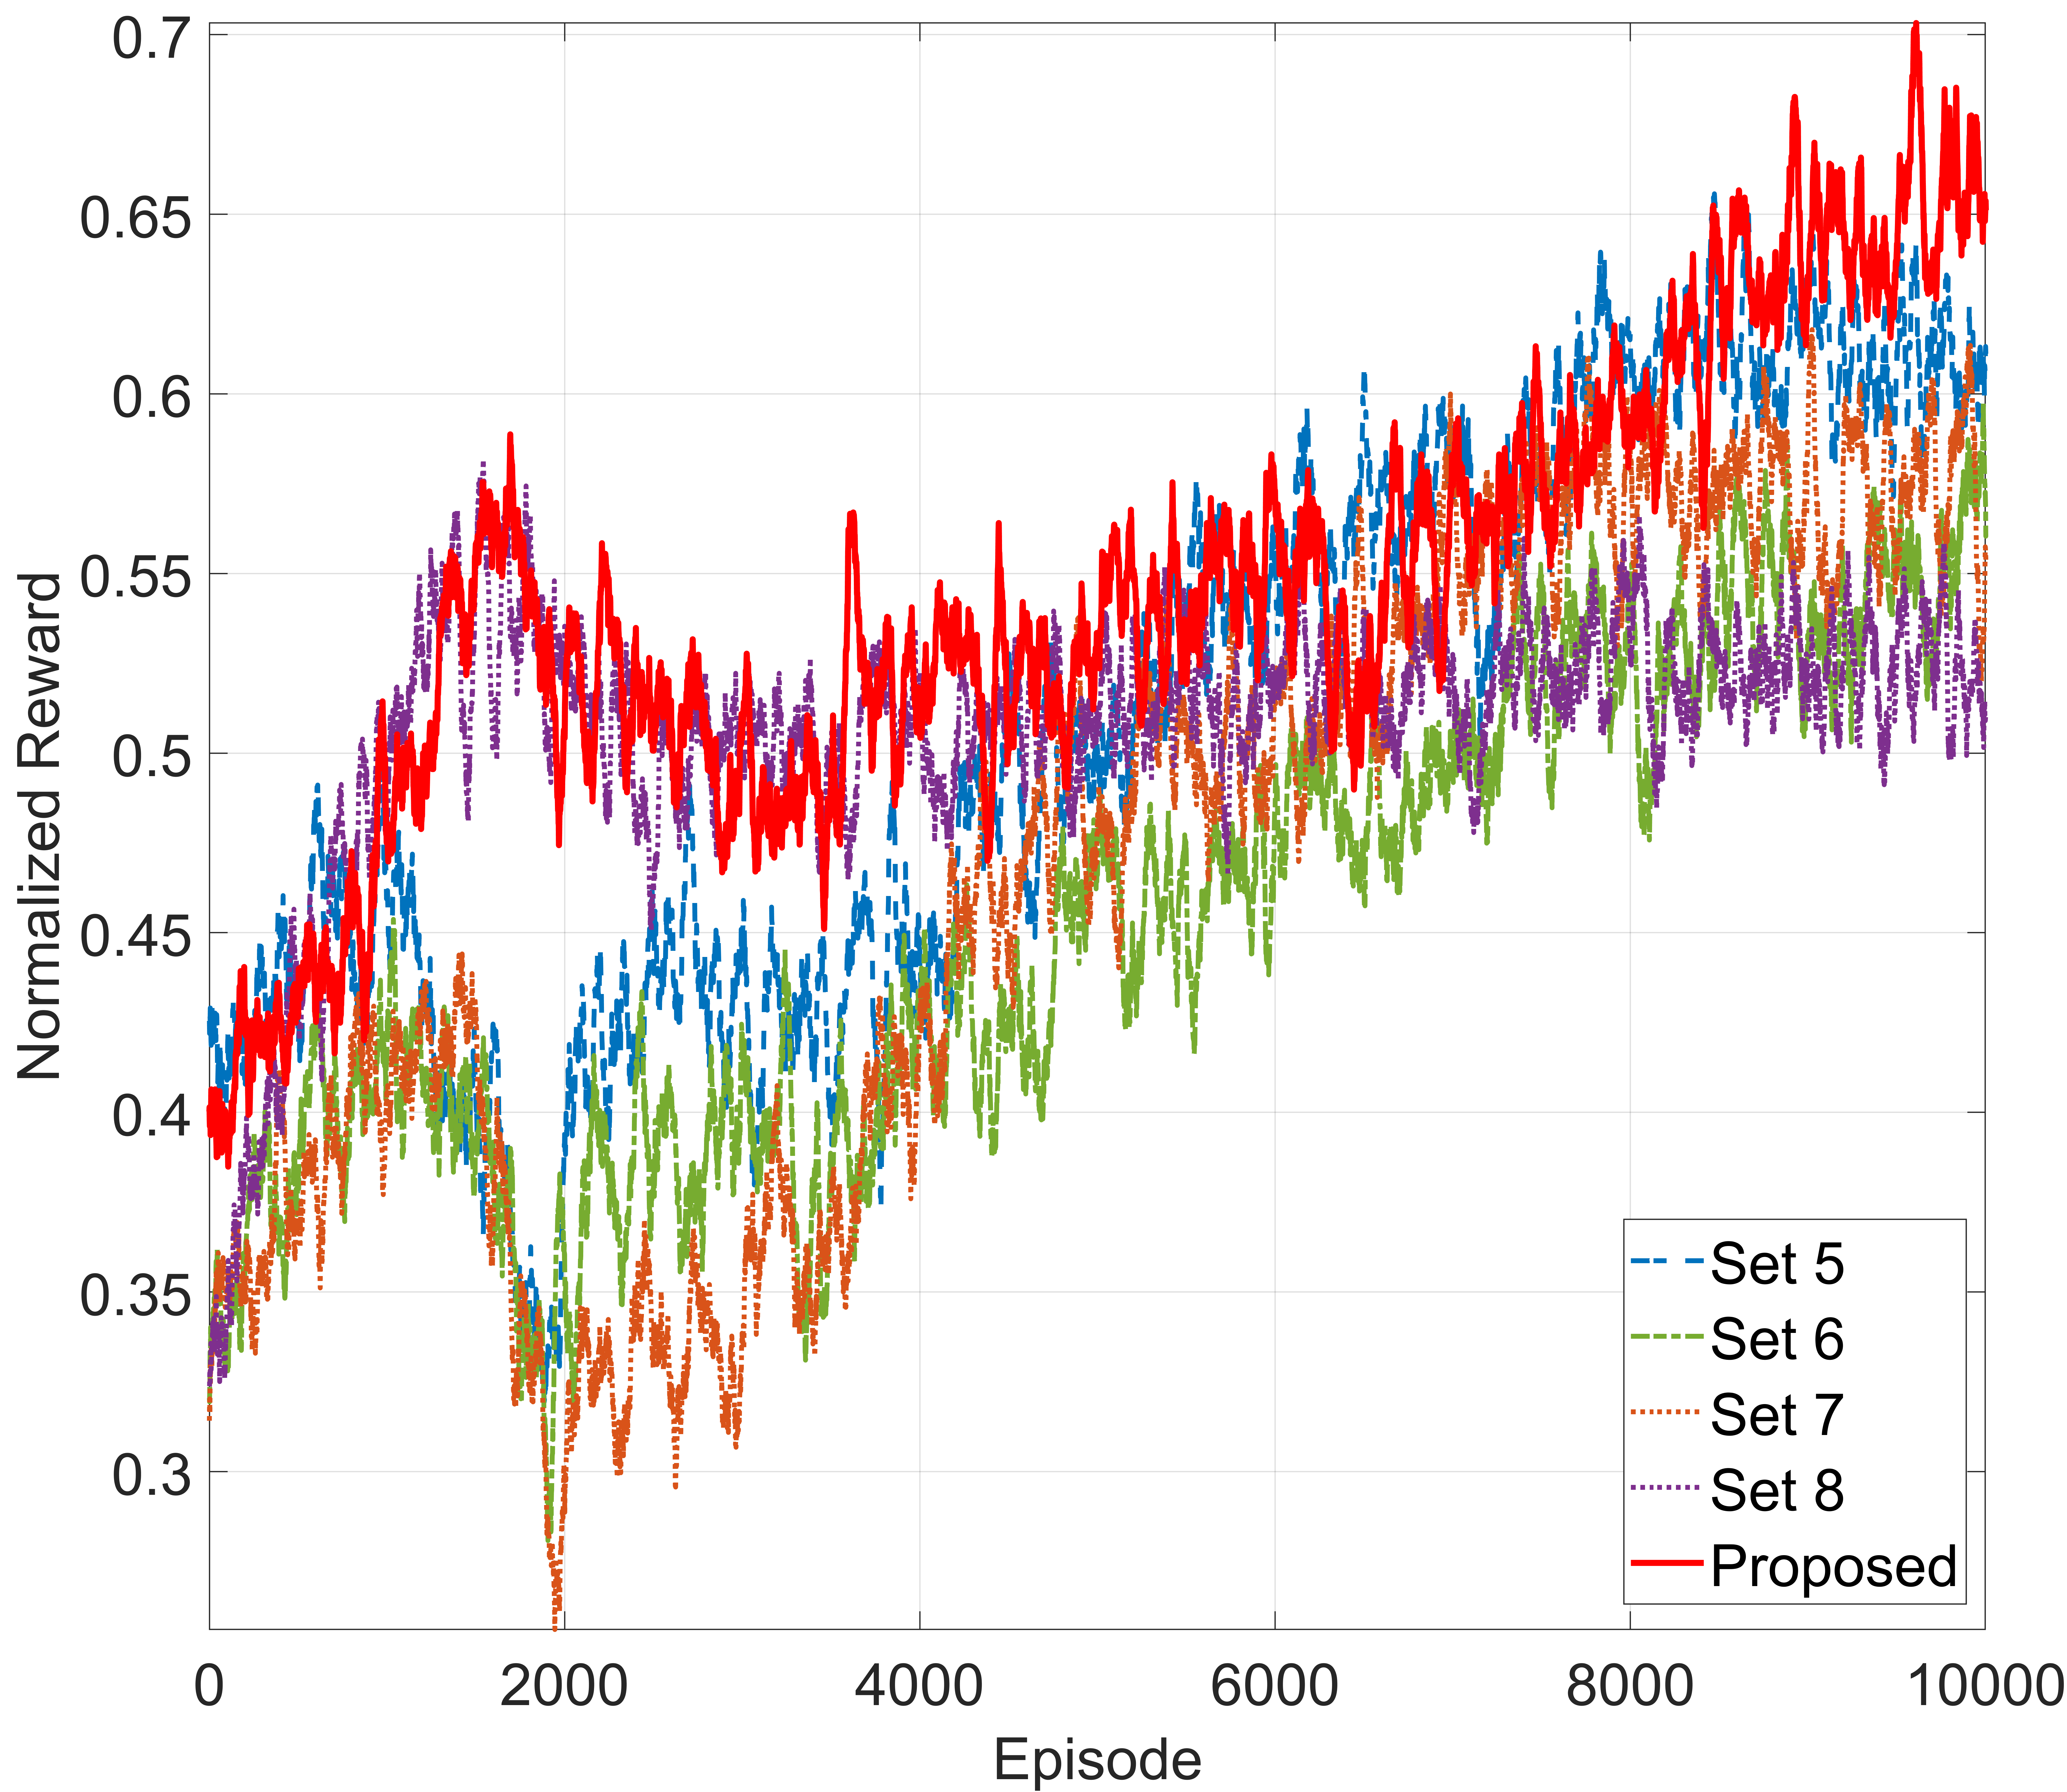
\includegraphics[width=\linewidth]{figure/reward.png}
    \caption{Normalized reward with 50 moving average comparison over episodes for the proposed algorithm and ablation baselines (Set~5--8).}
    \label{fig:reward}
\end{figure}
% 그림~\ref{fig:reward}는 제안된 Dueling DDQN 에이전트와 기준 체계(Set~5~8)에 대한 훈련 단계 동안의 정규화된 평균 보상의 수렴을 보여줍니다. 결과는 각 알고리즘 구성 요소가 학습 안정성과 최종 성능에 미치는 뚜렷한 영향을 보여줍니다. 제안된 알고리즘은 가장 높은 점근적 보상을 달성하고 초기 탐색 단계 이후 가장 안정적인 수렴 궤적을 보여줍니다. 이는 Dueling 아키텍처, PER 및 Polyak 평균화를 통합하는 것이 ToS 및 RSRP를 최대화하는 동시에 FLSO 빈도 및 부하 분산을 최소화하는 등 여러 목표 간의 균형을 효과적으로 맞춘다는 것을 확인시켜 줍니다. 대조적으로, 절제 연구는 각 구성 요소의 필요성을 강조합니다. Set~7은 에피소드 2,000 근처에서 치명적인 성능 붕괴를 겪습니다. 이는 우선 순위 샘플링 없이는 에이전트가 드물지만 중요한 부정적인 경험으로부터 효율적으로 학습하지 못하여 느린 회복 전에 일시적인 정책 저하로 이어진다는 것을 나타냅니다. Set~8은 빠른 초기 학습을 보여주지만 제안된 방법에 비해 훨씬 낮은 보상 수준에서 포화됩니다. 이는 타겟 네트워크의 "하드 업데이트"가 훈련 불안정성을 유발하여 에이전트가 최적의 GW 선택을 위해 정책을 미세 조정하는 것을 방해함을 시사합니다. 또한 표준 Set~5와 Set~6은 합리적인 학습 경향을 보이지만 제안된 방법보다 더 높은 분산과 낮은 최종 보상을 나타냅니다. 구체적으로 Set~6은 상당한 변동을 겪으며, 이는 Dueling 아키텍처가 LEO 위성 네트워크의 복잡한 상태 공간에서 가치 추정을 안정화하는 데 중요하다는 것을 의미합니다. 

\begin{figure}[t]
    \centering
    \includegraphics[width=\linewidth]{figure/1.flso.png}
    \caption{Average FLSO per each GW link for the proposed algorithm and baselines across different simulation steps.}
    \label{fig:1.flso}
\end{figure}

Fig.~\ref{fig:1.flso} shows the evolution of the average FLSO rate per GW link as the simulation progresses from 100 to 500 steps. Across all algorithms the FLSO count increases approximately linearly with the number of steps, and the relative ordering between aggressive and conservative strategies remains consistent at every time scale. Set~1 shows the most aggressive behavior, rising from 4.34 FLSOs at 100 steps to 16.99 at 500 steps, while Set~2 with a larger hysteresis margin grows from 3.17 to 11.55. The hard update RL variant in Set~8 follows a similar trend, rising from 2.92 to 10.52, which confirms that both small hysteresis and naive policy updates lead to persistent ping pong effects and unstable connectivity over long time scales. Distance based heuristics in Set~3 and Set~4 show more conservative behavior, evolving from around 2.10 to 8.73 and from 2.10 to 8.40 respectively. The standard RL baselines in Set~5, Set~6 and Set~7 remain in a comparable range, reaching 7.95, 8.46 and 7.75 FLSOs at 500 steps. The Random policy yields a relatively flat and moderate increase from 2.81 to 7.96 but does so without explicitly optimizing link quality or load balancing. The proposed algorithm consistently maintains a moderate switching rate across all time scales, growing from 1.82 at 100 steps to 7.98 at 500 steps, which is close to or lower than the more conservative baselines while still actively reacting to link quality. This trajectory demonstrates that the proposed method avoids the excessive switching of aggressive signal based schemes not only at the end of the simulation but throughout the entire period, while performing enough FLSOs to preserve load balancing and link quality that the Random policy cannot guarantee.
% 그림~\ref{fig:1.flso}는 시뮬레이션이 100단계에서 500단계로 진행됨에 따라 GW 링크당 평균 FLSO 비율의 변화를 나타냅니다. 모든 알고리즘에서 FLSO 수는 단계 수에 따라 대략 선형적으로 증가하며, 공격적 및 보수적 전략 간의 상대적 순서는 모든 시간 척도에서 일관되게 유지됩니다. Set~1은 가장 공격적인 동작을 보여 100단계에서 4.34 FLSO에서 500단계에서 16.99로 상승하며, 더 큰 히스테리시스 마진을 가진 Set~2는 3.17에서 11.55로 증가합니다. Set~8의 "하드 업데이트" RL 변형은 유사한 추세를 따르며 2.92에서 10.52로 상승하여 작은 히스테리시스와 순진한 정책 업데이트가 모두 장기적인 핑퐁 효과와 불안정한 연결성으로 이어진다는 것을 확인시켜 줍니다. Set~3과 Set~4의 거리 기반 휴리스틱은 각각 약 2.10에서 8.73 및 2.10에서 8.40으로 진화하며 더 보수적인 동작을 보여줍니다. Set~5, Set~6 및 Set~7의 표준 RL 기준 체계는 유사한 범위에 머물며 500단계에서 각각 7.95, 8.46 및 7.75 FLSO에 도달합니다. 무작위 정책은 상대적으로 평탄하고 완만한 증가를 보여주지만(2.81에서 7.96) 링크 품질이나 부하 분산을 명시적으로 최적화하지 않습니다. 제안된 알고리즘은 모든 시간 척도에서 일관되게 적당한 스위칭 속도를 유지하며, 100단계에서 1.82에서 500단계에서 7.98로 성장하여 더 보수적인 기준 체계와 비슷하거나 낮으면서도 여전히 링크 품질에 적극적으로 반응합니다. 이 궤적은 제안된 방법이 시뮬레이션 종료 시점뿐만 아니라 전체 기간 동안 공격적인 신호 기반 스킴의 과도한 스위칭을 피하면서 무작위 정책이 보장할 수 없는 부하 분산 및 링크 품질을 유지하기 위해 충분한 FLSO를 수행함을 보여줍니다.

\begin{figure}[t]
    \centering
    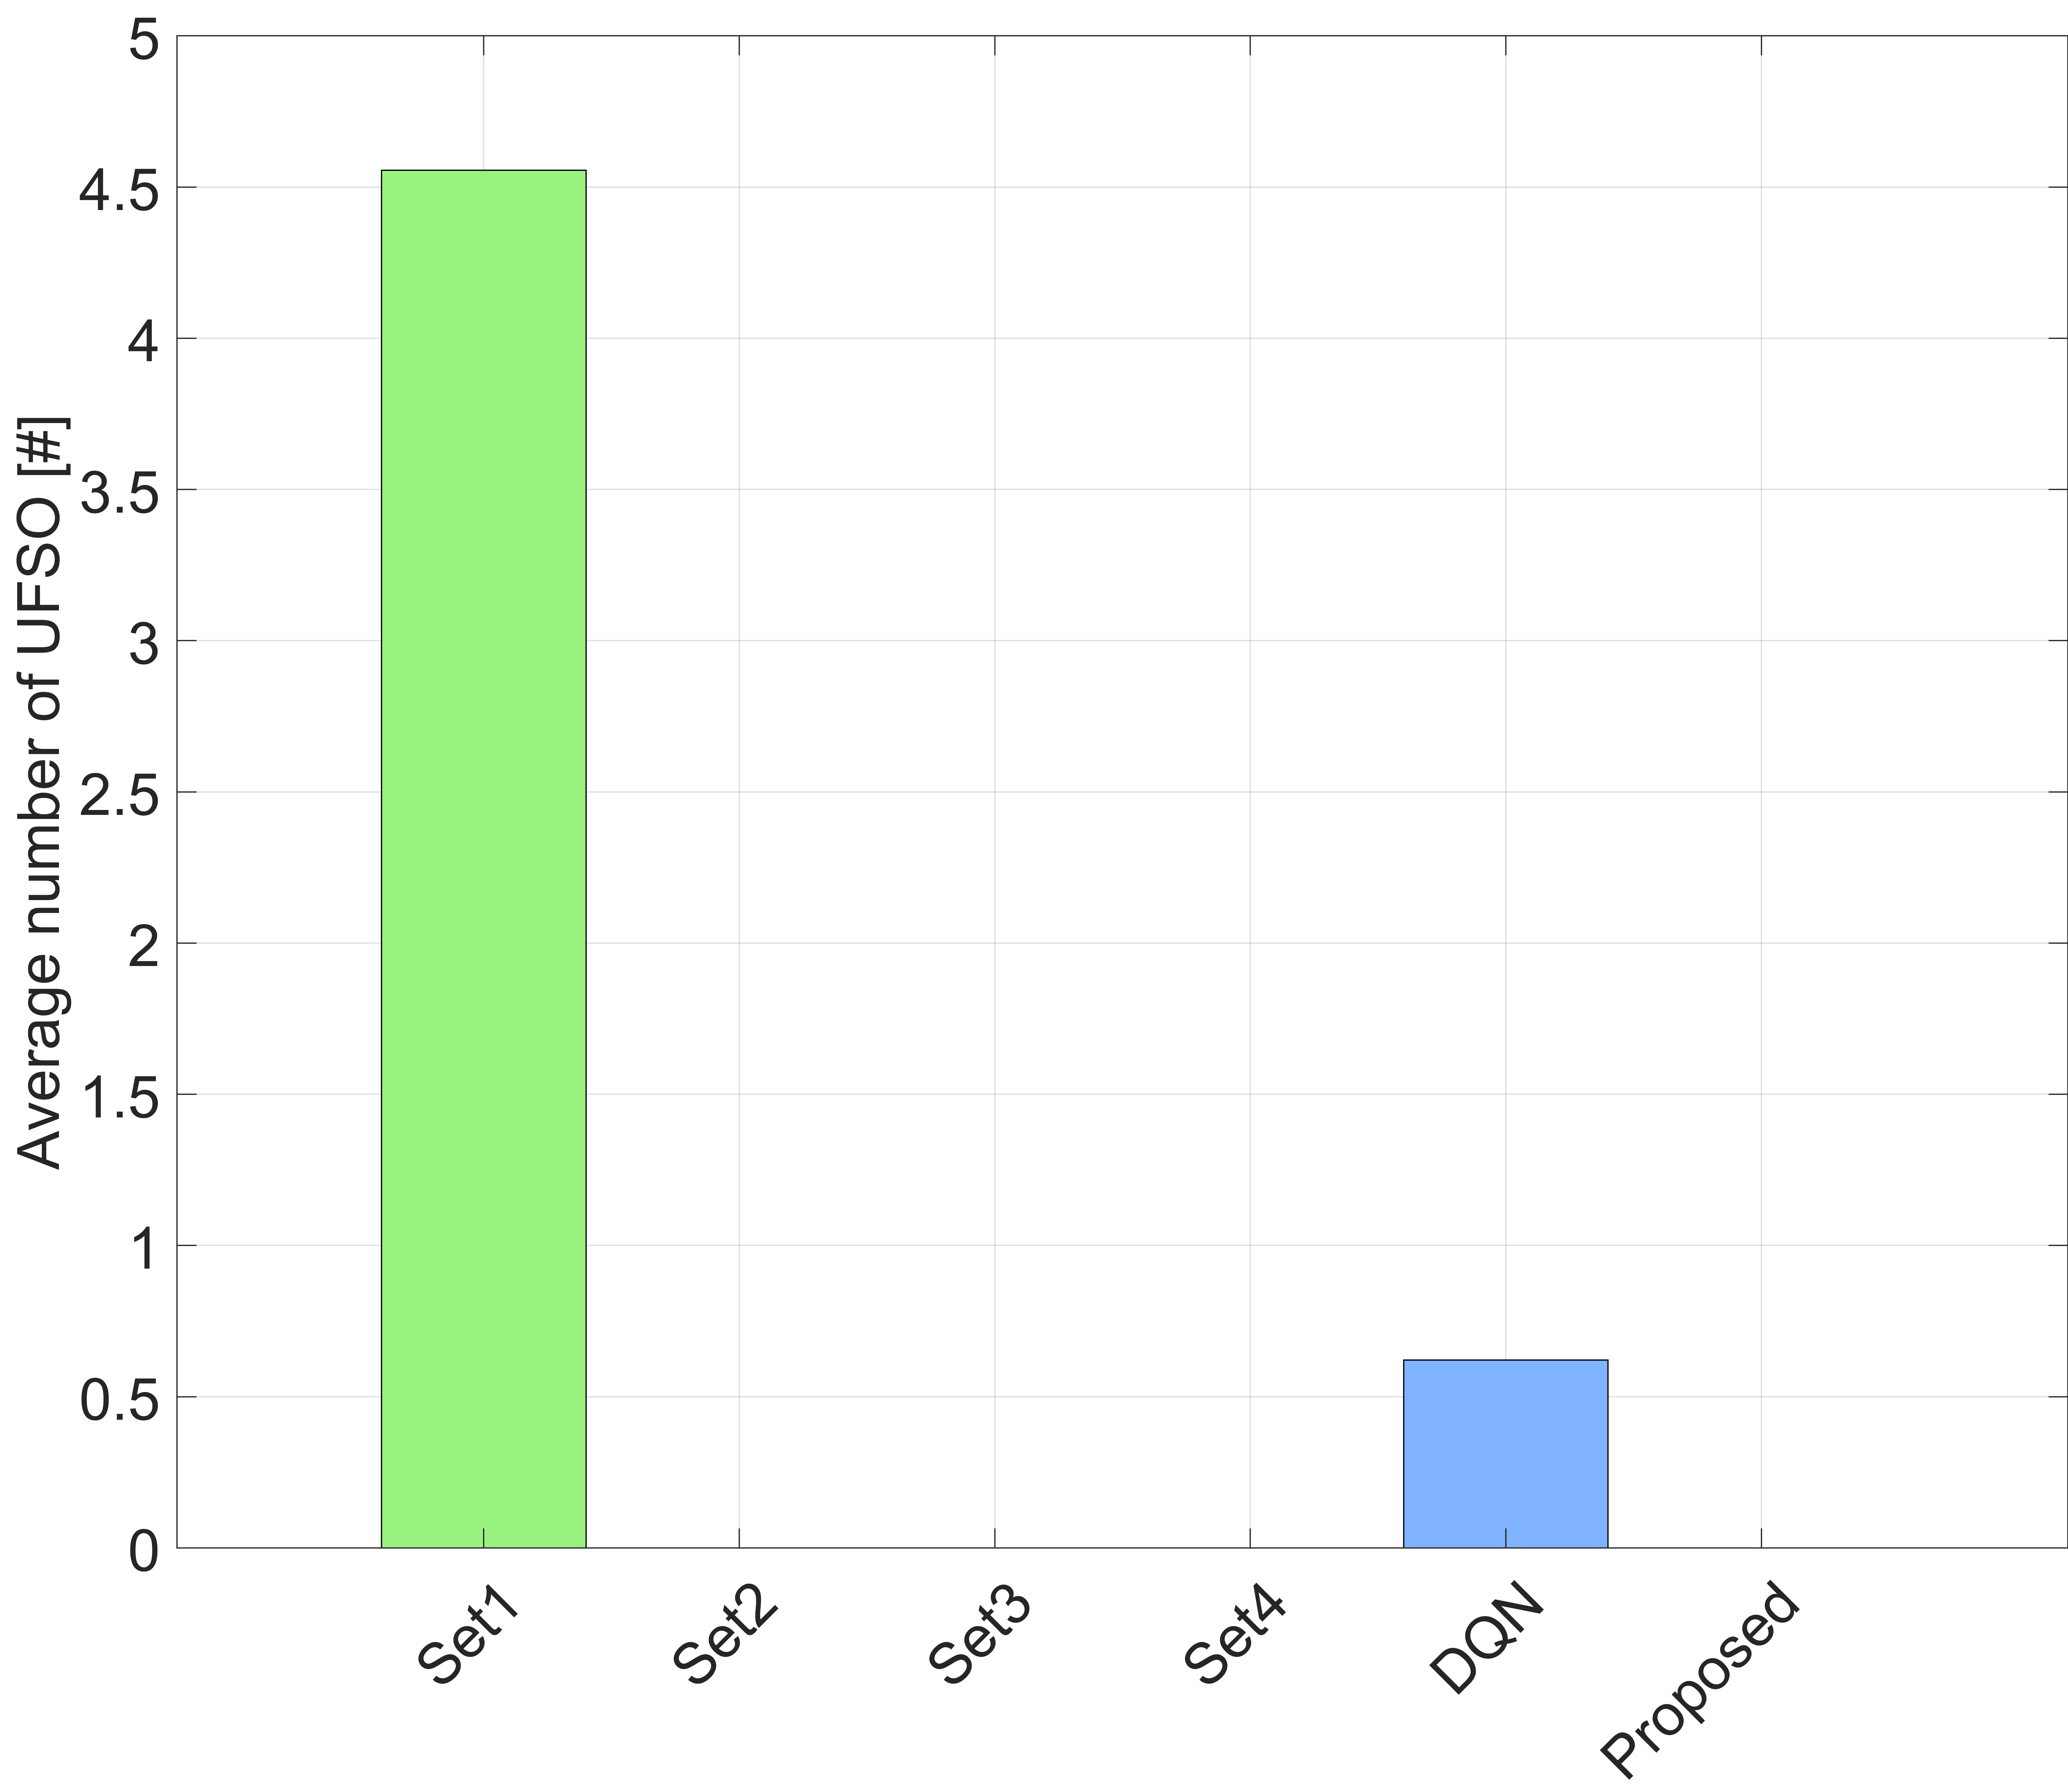
\includegraphics[width=\linewidth]{figure/2.ufso.png}
    \caption{Average UFLSO per each GW link for the proposed algorithm and baselines across different simulation steps.}
    \label{fig:2.ufso}
\end{figure}

Fig.~\ref{fig:2.ufso} presents the evolution of the average UFLSO count as a function of the simulation length from 100 to 500 steps. For all algorithms the UFLSO increases almost linearly with the number of steps, and the relative ordering between aggressive and conservative strategies remains stable over time. Set~1 yields the largest UFLSO values, rising from about 0.88 at 100 steps to 5.09 at 500 steps. This shows that the frequent FLSOs generated by a small hysteresis margin translate into a large number of unstable and ultimately harmful switching operations. Set~2 reduces the UFLSO growth but still reaches 2.94 at 500 steps, which indicates that enlarging the hysteresis margin alone is not sufficient to fully stabilize the FLSO process. Distance based heuristics in Set~3 and Set~4 exhibit clearly more conservative behaviour. Their UFLSO values grow from roughly 0.24 at 100 steps to 2.41 and from 0.23 to 2.18 at 500 steps. These curves confirm that limiting switching decisions to geometric criteria suppresses unstable transitions more effectively than purely signal driven triggering. RL baselines Set~5, Set~6, and Set~7 occupy an intermediate region. Their final UFLSO values range from 2.75 in Set~5 to 3.26 in Set~6, which is lower than the aggressive signal based Set~1 and the hard update RL variant Set~8, but still clearly higher than the distance based heuristics. Set~8, which adopts hard and infrequent target updates in the RL pipeline, shows UFLSO growth from about 1.44 to 4.32 and thus remains close to Set~1 in terms of instability. This behaviour confirms that naive RL update rules do not provide sufficient regularization of the switching pattern. The Random policy produces UFLSO values between 1.14 and 2.52 over the considered range. Although this level is moderate, the corresponding controller does not exploit link quality or load balancing in a principled way, as shown by the throughput and fairness metrics. The proposed algorithm maintains a consistently low UFLSO rate over the entire simulation horizon. Its UFLSO increases from 0.69 at 100 steps to 2.51 at 500 steps, which places it very close to Set~3 and Set~4 and well below Set~1, Set~2, Set~5, Set~6, Set~7, and Set~8 at every time scale. At the final step the UFLSO of the proposed method is comparable to that of the Random policy, yet the proposed controller simultaneously achieves much higher throughput and better load balancing. Overall, the UFLSO results demonstrate that the proposed algorithm suppresses unstable switching events to approximately half the level of the most aggressive signal based and hard update RL schemes, while preserving a stability profile that matches or slightly improves upon carefully tuned distance based heuristics.
% 그림~\ref{fig:2.ufso}는 시뮬레이션 길이(100단계에서 500단계까지)의 함수로서 평균 UFLSO 수의 변화를 나타냅니다. 모든 알고리즘에서 UFLSO는 단계 수에 따라 거의 선형적으로 증가하며, 공격적 및 보수적 전략 간의 상대적 순서는 시간이 지나도 안정적으로 유지됩니다. Set~1은 100단계에서 약 0.88에서 500단계에서 5.09로 상승하여 가장 큰 UFLSO 값을 산출합니다. 이는 작은 히스테리시스 마진으로 생성된 빈번한 FLSO가 불안정하고 궁극적으로 해로운 스위칭 작업의 많은 수로 이어진다는 것을 보여줍니다. Set~2는 UFLSO 성장을 줄이지만 여전히 500단계에서 2.94에 도달하여 히스테리시스 마진을 늘리는 것만으로는 핸드오버 프로세스를 완전히 안정화하기에 충분하지 않음을 나타냅니다. Set~3과 Set~4의 거리 기반 휴리스틱은 명확히 더 보수적인 동작을 보입니다. 그들의 UFLSO 값은 100단계에서 대략 0.24에서 500단계에서 2.41로, 그리고 0.23에서 2.18로 증가합니다. 이러한 곡선은 기하학적 기준으로 스위칭 결정을 제한하는 것이 순수하게 신호 기반 트리거링보다 불안정한 전환을 더 효과적으로 억제한다는 것을 확인시켜 줍니다. RL 기준 체계 Set~5, Set~6, 및 Set~7은 중간 영역을 차지합니다. 그들의 최종 UFLSO 값은 Set~5에서 2.75에서 Set~6에서 3.26까지 범위에 있으며, 이는 공격적인 신호 기반 Set~1 및 "하드 업데이트" RL 변형 Set~8보다 낮지만 여전히 거리 기반 휴리스틱보다 명확히 높습니다. RL 파이프라인에서 하드하고 드문 타겟 업데이트를 채택하는 Set~8은 약 1.44에서 4.32로 UFLSO 성장을 보여주며 불안정성 측면에서 Set

\begin{figure}[t]
    \centering
    \includegraphics[width=\linewidth]{figure/3.tos.png}
    \caption{Average ToS per each GW link for the proposed algorithm and baselines across different simulation steps.}
    \label{fig:3.tos}
\end{figure}

Fig.~\ref{fig:3.tos} shows the evolution of the total offered service ToS as the number of simulation steps increases from 100 to 500. For all algorithms the ToS grows monotonically with the simulation length, and the relative ordering between the schemes remains consistent over time. The signal based baselines in Set~1 and Set~2 exhibit the lowest throughput region. Their curves start around fifteen to seventeen at 100 steps and reach only about twenty five and thirty two at 500 steps, which indicates that aggressive reliance on instantaneous signal strength alone does not fully exploit the available network capacity. Distance based heuristics in Set~3 and Set~4 achieve significantly higher ToS. At 100 steps they already provide more than twenty units of service and continue to increase toward approximately forty four at 500 steps. This demonstrates that even without explicit learning, a carefully designed geometric policy can sustain much higher long term throughput than simple signal driven hysteresis rules. The hard update RL variant in Set~8 lies between these two groups, rising from roughly sixteen at 100 steps to about thirty four at 500 steps, which suggests that naive design of the value update mechanism underutilizes the potential of reinforcement learning. RL baselines in Set~5, Set~6, and Set~7 form the top throughput group. Their ToS values start near thirty at 100 steps and grow to about forty seven, forty six, and fifty at 500 steps. These results confirm that well tuned RL controllers can aggressively exploit the available GW resources to maximize long term service. The Random policy produces a ToS curve that stays below the RL baselines and distance based heuristics. It increases from about sixteen at 100 steps to roughly thirty nine at 500 steps, which reflects the absence of any structured optimisation in its switching behaviour. The proposed algorithm closely tracks the best distance based heuristics in terms of ToS. It starts at about twenty four at 100 steps and rises steadily to approximately forty four at 500 steps, almost overlapping with Set~3 and Set~4 across the entire simulation horizon. Compared with the strongest RL baselines, the proposed method accepts a modest reduction in maximum throughput in exchange for the substantial gains in switching stability reported by the FLSO and UFLSO metrics. Combined with the traffic and fairness results, the ToS curves show that the proposed controller is able to sustain high long term service while avoiding the excessive switching overhead of the most agressive schemes.
 % 그림~ef{fig:3.tos}는 시뮬레이션 단계 수가 100에서 500으로 증가함에 따라 제공된 총 서비스 ToS의 변화를 보여줍니다. 모든 알고리즘에서 ToS는 시뮬레이션 길이에 따라 단조롭게 증가하며, 체계 간의 상대적 순서는 시간이 지나도 일관되게 유지됩니다. Set~1과 Set~2의 신호 기반 기준 체계는 가장 낮은 처리량 영역을 나타냅니다. 그들의 곡선은 100단계에서 약 15에서 17 사이에서 시작하여 500단계에서 약 25와 32에 도달하는데, 이는 순간적인 신호 강도에 대한 공격적인 의존만으로는 사용 가능한 네트워크 용량을 완전히 활용하지 못함을 나타냅니다. Set~3과 Set~4의 거리 기반 휴리스틱은 훨씬 더 높은 ToS를 달성합니다. 100단계에서 이미 20단위 이상의 서비스를 제공하며 500단계에서 약 44까지 계속 증가합니다. 이는 명시적인 학습 없이도 신중하게 설계된 기하학적 정책이 단순한 신호 기반 히스테리시스 규칙보다 훨씬 더 높은 장기 처리량을 유지할 수 있음을 보여줍니다. Set~8의 "하드 업데이트" RL 변형은 이 두 그룹 사이에 위치하며, 100단계에서 대략 16에서 시작하여 500단계에서 약 34로 상승하여 가치 업데이트 메커니즘의 순진한 설계가 강화 학습의 잠재력을 충분히 활용하지 못함을 시사합니다. Set~5, Set~6 및 Set~7의 RL 기준 체계는 최고 처리량 그룹을 형성합니다. 그들의 ToS 값은 100단계에서 거의 30 근처에서 시작하여 500단계에서 약 47, 46 및 50으로 증가합니다. 이러한 결과는 잘 조정된 RL 컨트롤러가 사용 가능한 게이트웨이 자원을 공격적으로 활용하여 장기 서비스를 극대화할 수 있음을 확인시켜 줍니다. 무작위 정책은 RL 기준 체계 및 거리 기반 휴리스틱 아래에 머무르는 ToS 곡선을 생성합니다. 그것은 100단계에서 약 16에서 시작하여 500단계에서 대략 39까지 증가하며, 이는 그 스위칭 동작에 구조화된 최적화가 없음을 반영합니다. 제안된 알고리즘은 ToS 측면에서 최고의 거리 기반 휴리스틱을 밀접하게 추적합니다. 그것은 100단계에서 약 24에서 시작하여 500단계에서 약 44까지 꾸준히 상승하며 전체 시뮬레이션 기간 동안 거의 Set~3 및 Set~4와 겹칩니다. 가장 강력한 RL 기준 체계와 비교할 때, 제안된 방법은 FLSO 및 UFLSO 메트릭에서 보고된 상당한 스위칭 안정성 향상을 대가로 최대 처리량에서 겸손한 감소를 수용합니다. 트래픽 및 공정성 결과와 결합하여 ToS 곡선은 제안된 컨트롤러가 가장 공격적인 스위칭 오버헤드를 피하면서 높은 장기 서비스를 지속할 수 있음을 보여줍니다.

\begin{figure}[t]
    \centering
    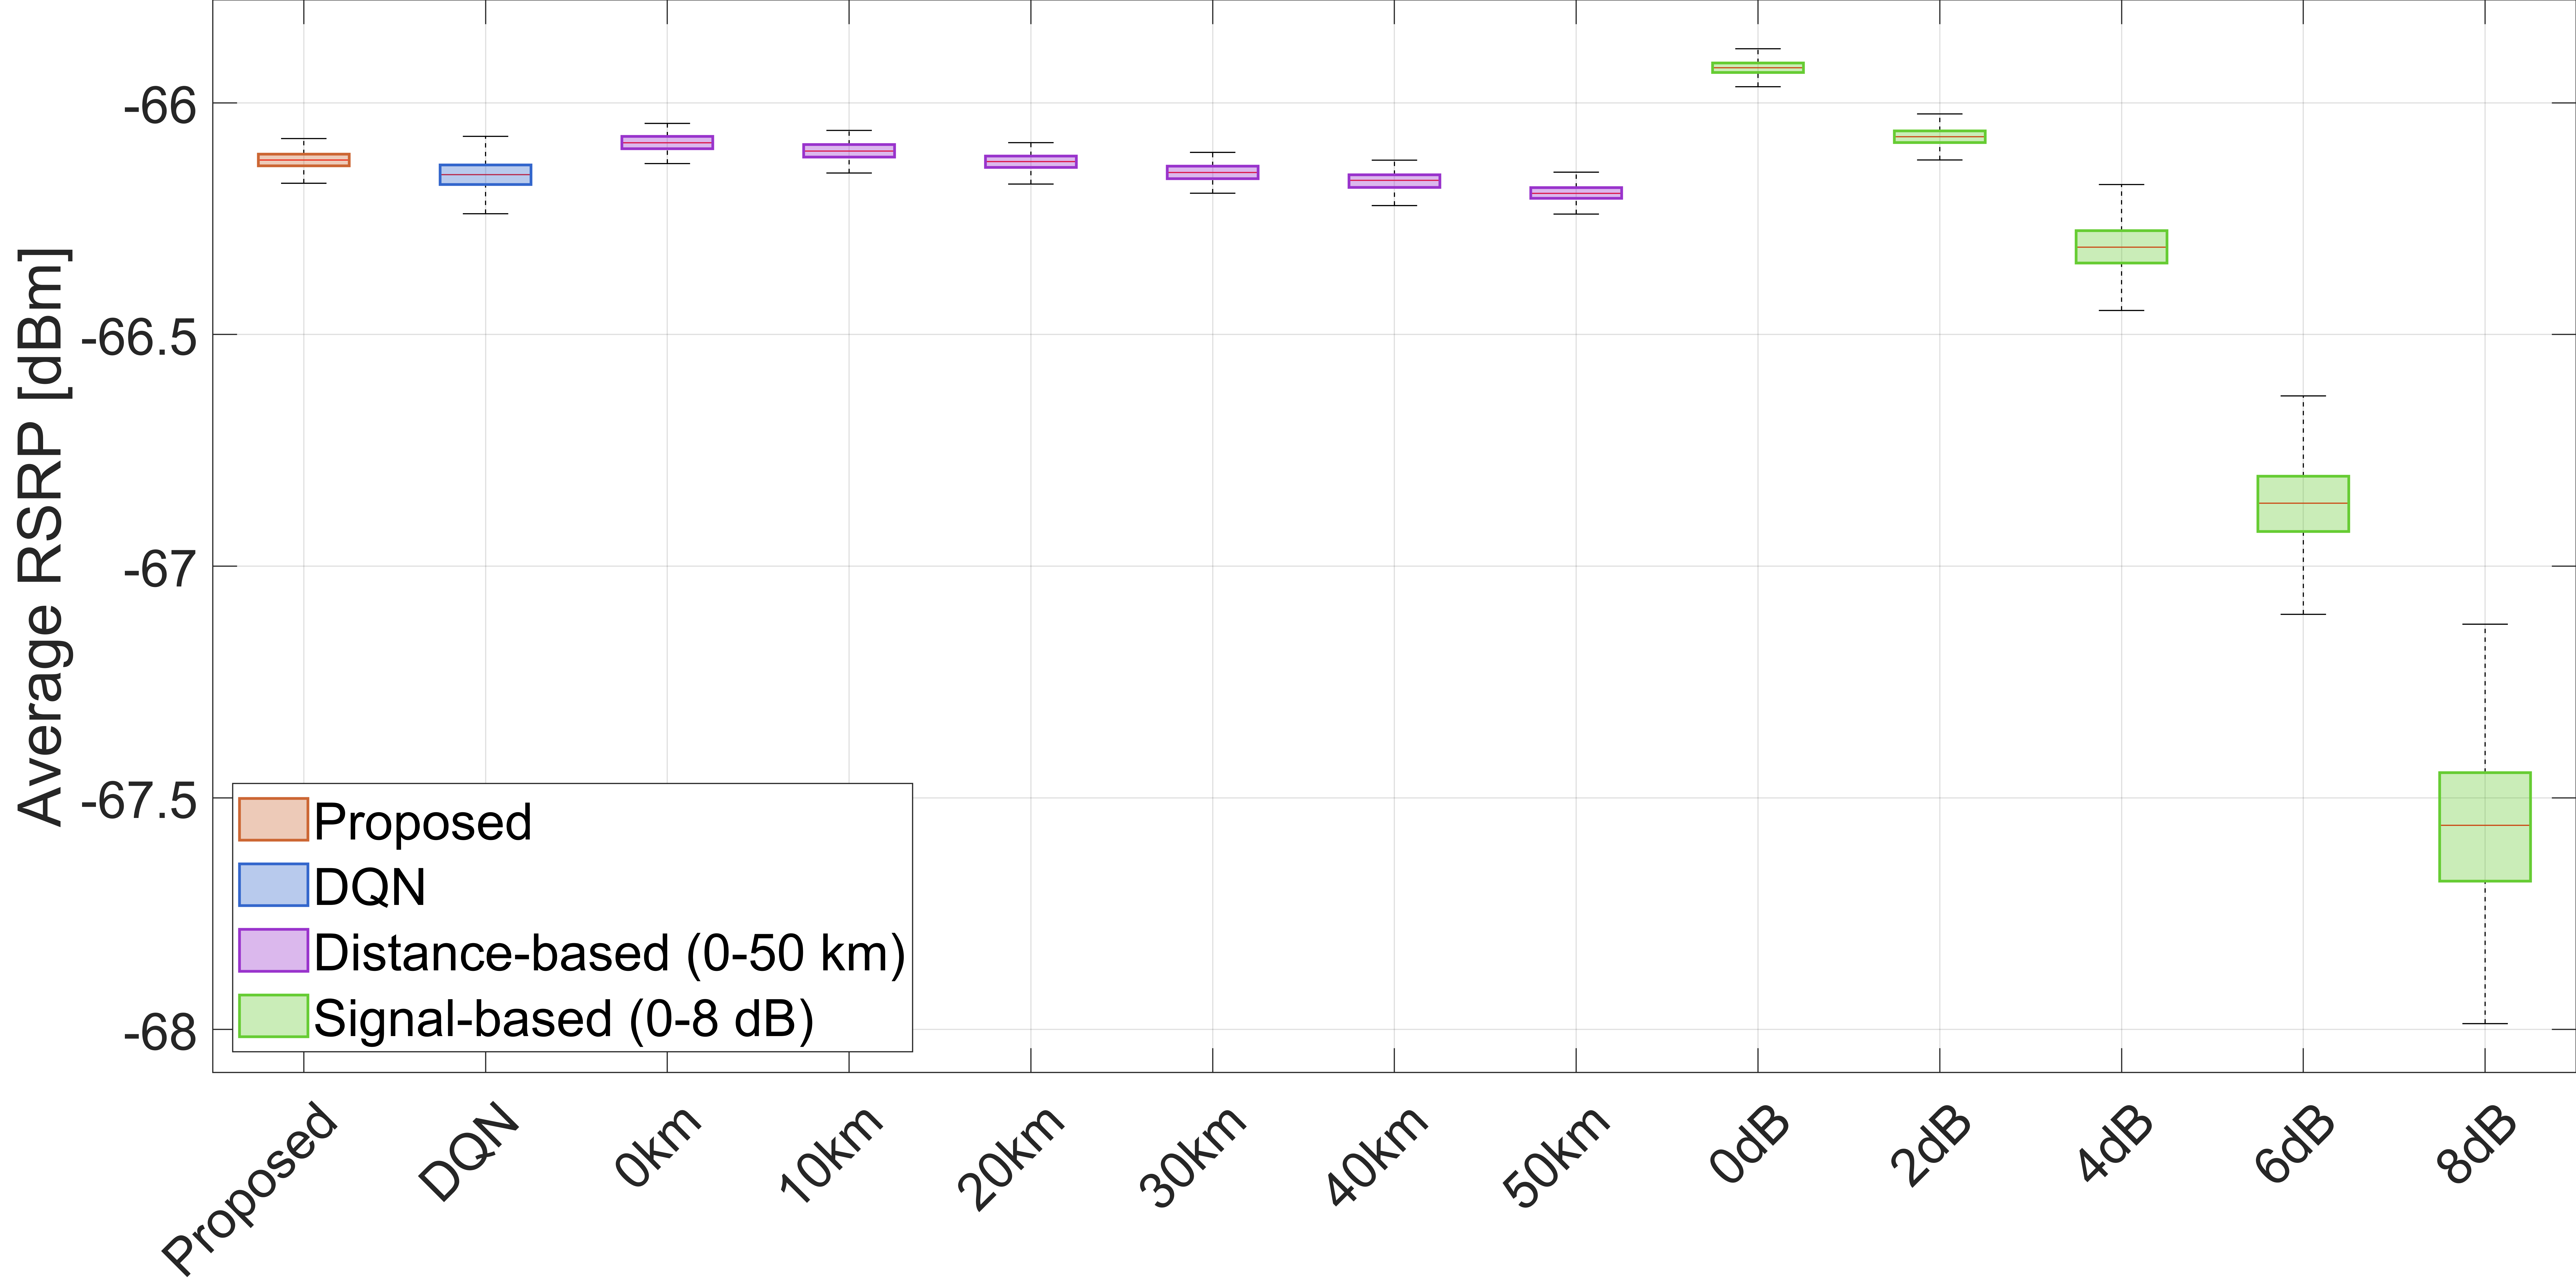
\includegraphics[width=\linewidth]{figure/4.rsrp.png}
    \caption{Average RSRP per GW for the proposed algorithm and baselines across different simulation steps.}
    \label{fig:4.rsrp}
\end{figure}

Fig.~\ref{fig:4.rsrp} shows the evolution of the average RSRP for all algorithms as the number of simulation steps increases from 100 to 500. The signal based schemes in Set~1 and Set~2 maintain the highest link quality, with average RSRP values around \(-55\) dB and only very small variations over time. This behaviour confirms that aggressive signal driven switching is effective at keeping each satellite attached to the currently strongest GW. Distance based heuristics in Set~3 and Set~4 exhibit clearly lower RSRP levels. Their averages degrade from about \(-58\) dB at 100 steps to around \(-59.2\) dB at 500 steps, which indicates that geometric criteria alone cannot consistently select the strongest links. The RL baselines in Set~5, Set~6, and Set~7 and the proposed algorithm form an intermediate group with average RSRP values between roughly \(-58.4\) dB and \(-58.9\) dB at the end of the simulation. Within this group the proposed method closely follows Set~5 and Set~6 and maintains a very stable RSRP trajectory across all time scales. The Random policy starts from about \(-56.8\) dB at 100 steps and gradually converges toward \(-58.2\) dB at 500 steps, which is slightly better than the proposed method in terms of pure signal strength but is achieved without any explicit optimisation of load balancing or switching stability. Overall, the proposed controller accepts a moderate loss of approximately 3 dB compared with the strongest signal based schemes in order to obtain the substantial reductions in FLSO and UFLSO reported earlier, while preserving link quality comparable to other RL based approaches.
% 그림 ~\ref{fig:4.rsrp}는 시뮬레이션 단계 수가 100에서 500으로 증가함에 따라 모든 알고리즘에 대한 평균 RSRP의 변화를 보여줍니다. Set~1과 Set~2의 신호 기반 스킴은 평균 RSRP 값이 약 -55dB이고 시간에 따른 매우 작은 변동만 있는 최고 링크 품질을 유지합니다. 이러한 동작은 공격적인 신호 기반 스위칭이 각 위성을 현재 가장 강한 게이트웨이에 연결 상태로 유지하는 데 효과적임을 확인시켜 줍니다. Set~3과 Set~4의 거리 기반 휴리스틱은 명확히 낮은 RSRP 수준을 나타냅니다. 그들의 평균은 100단계에서 약 -58dB에서 500단계에서 약 -59.2dB로 저하되며, 이는 기하학적 기준만으로는 일관되게 가장 강한 링크를 선택할 수 없음을 나타냅니다. Set~5, Set~6, 및 Set~7의 RL 기준 체계와 제안된 알고리즘은 시뮬레이션 종료 시점에서 대략 -58.4dB와 -58.9dB 사이의 평균 RSRP 값을 가진 중간 그룹을 형성합니다. 이 그룹 내에서 제안된 방법은 Set~5 및 Set~6을 밀접하게 따르며 모든 시간 척도에서 매우 안정적인 RSRP 궤적을 유지합니다. 무작위 정책은 100단계에서 약 -56.8dB에서 시작하여 500단계에서 점차 -58.2dB로 수렴하며, 이는 순수한 신호 강도 측면에서 제안된 방법보다 약간 더 좋지만 부하 분산이나 스위칭 안정성의 명시적인 최적화 없이 달성됩니다. 전반적으로 제안된 컨트롤러는 앞서 보고된 FLSO 및 UFLSO의 상당한 감소를 얻기 위해 가장 강력한 신호 기반 스킴과 비교하여 약 3dB의 적당한 손실을 수용하면서 다른 RL 기반 접근 방식과 비교할 수 있는 링크 품질을 유지합니다.

\begin{figure}[t]
    \centering
    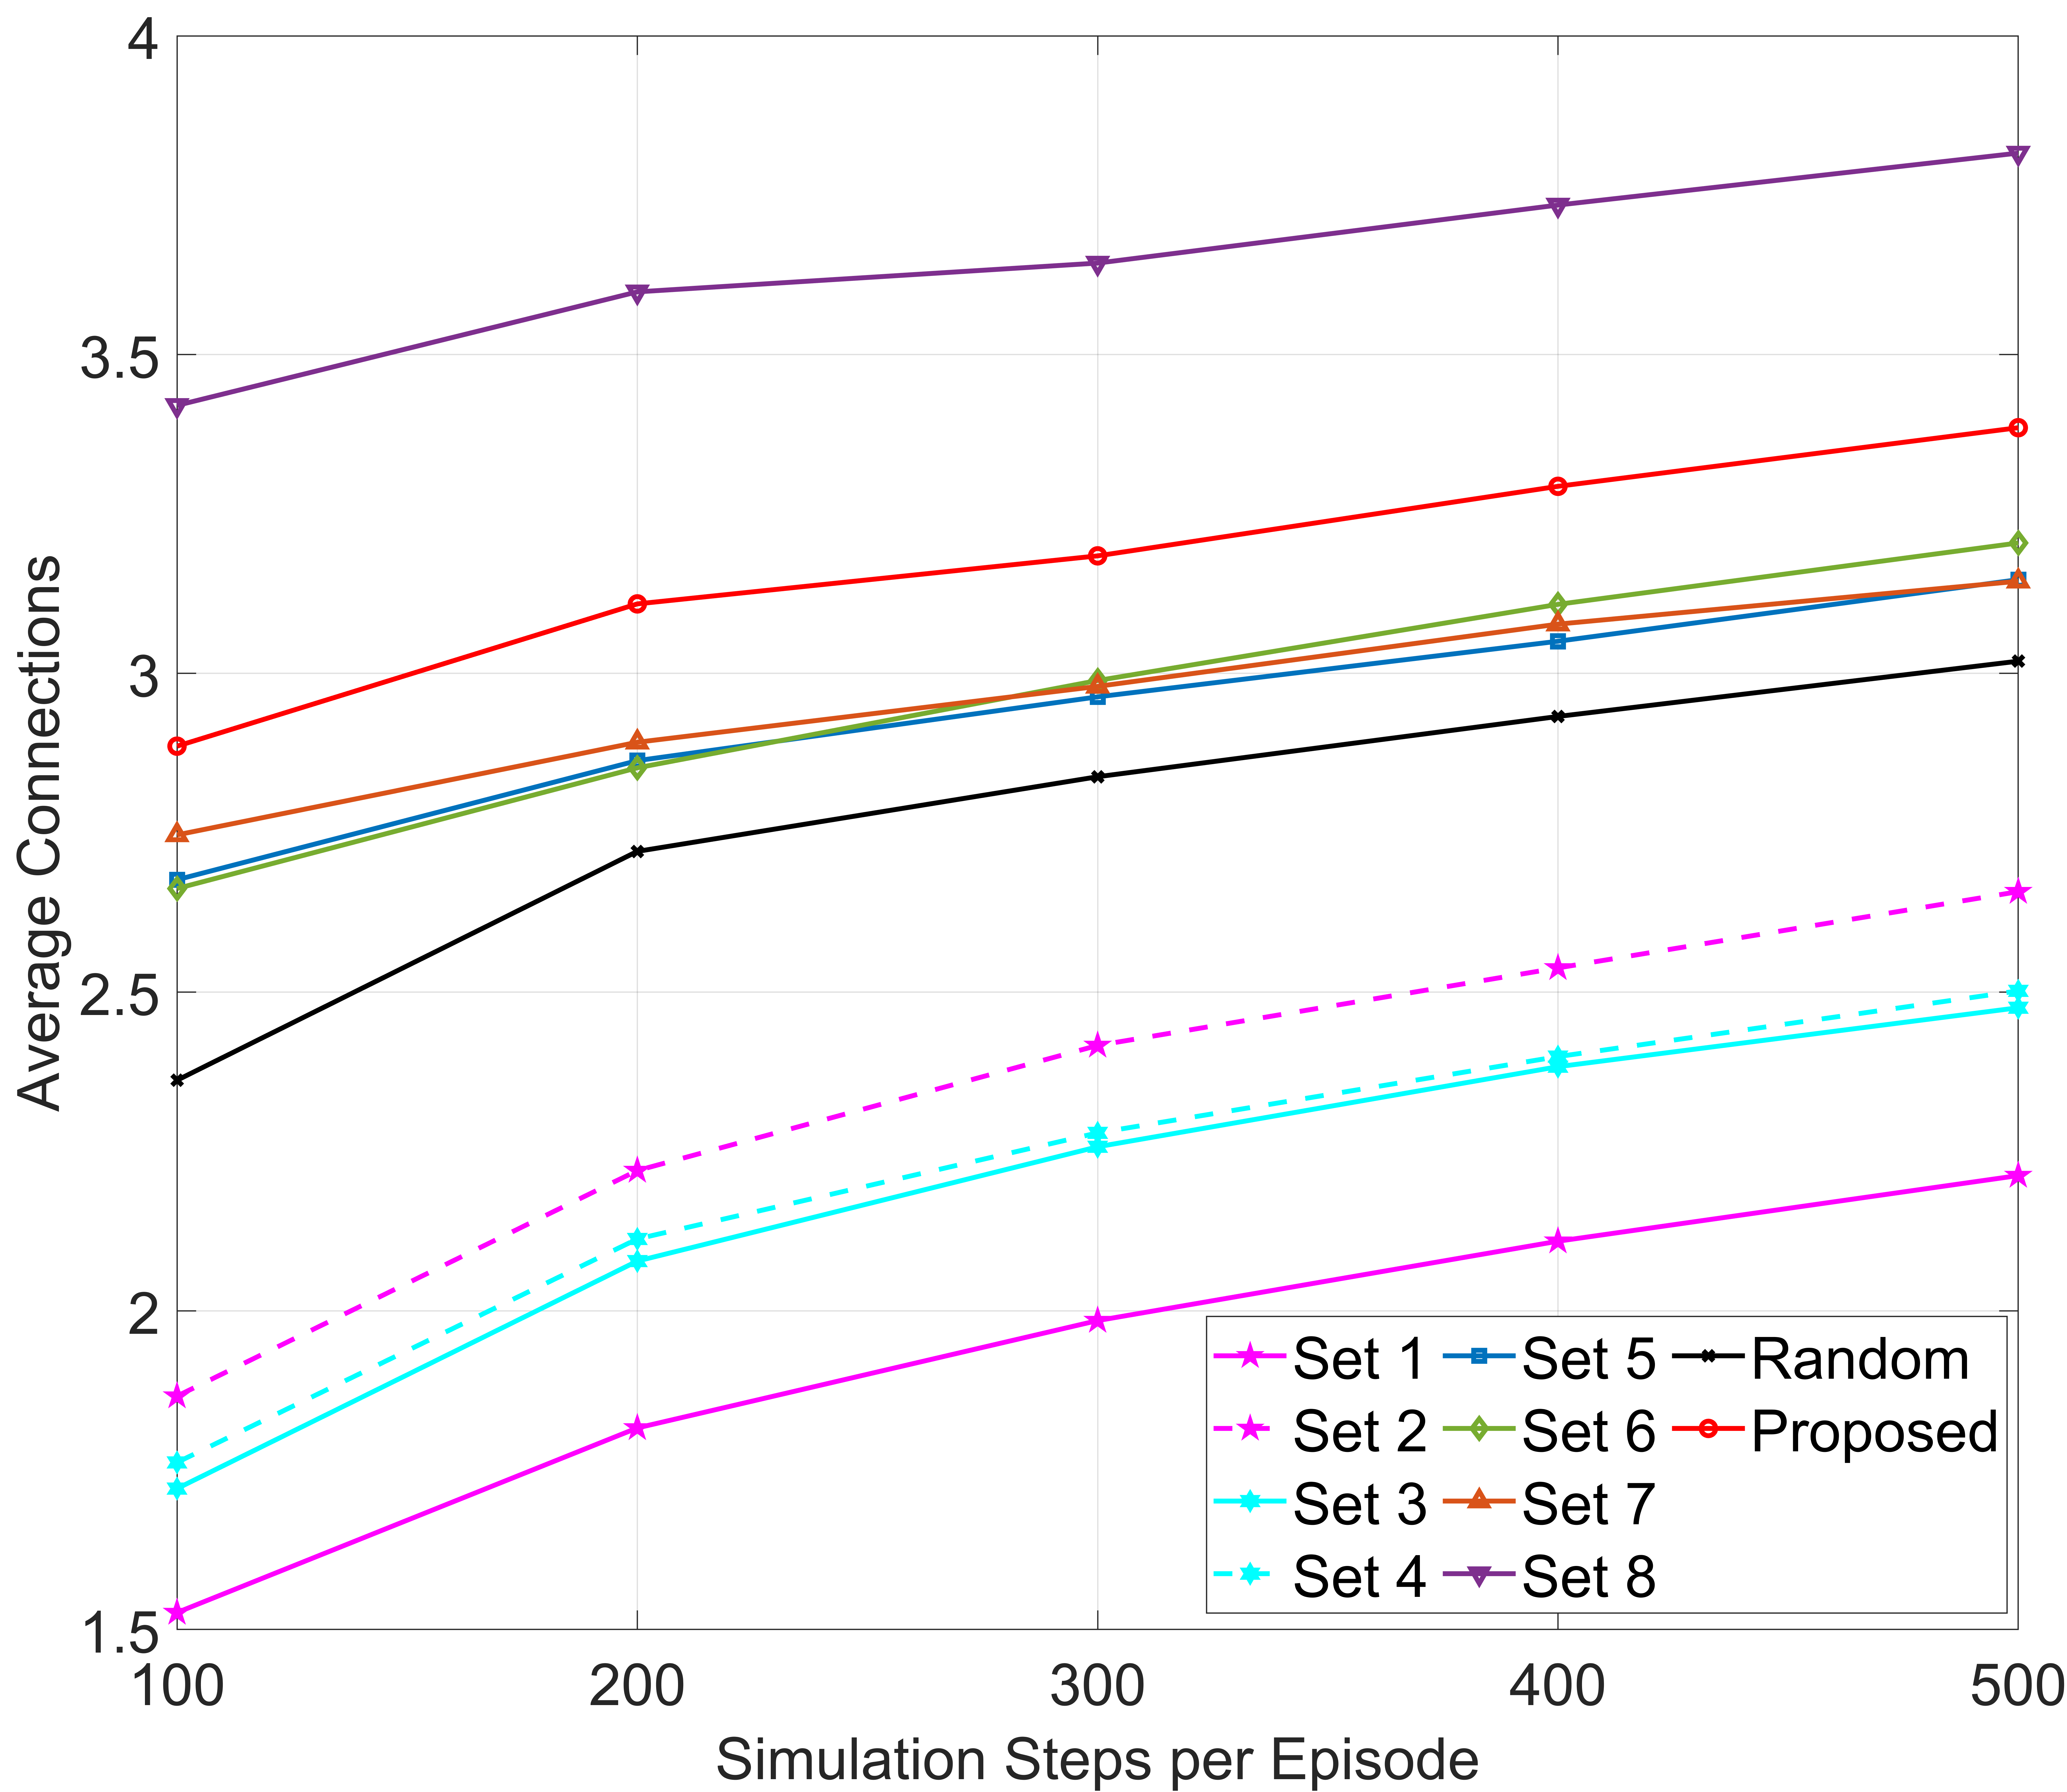
\includegraphics[width=\linewidth]{figure/5.connection.png}
    \caption{Average number of connections per GW for the proposed algorithm and baselines across different simulation steps.}
    \label{fig:5.connection}
\end{figure}

Fig.~\ref{fig:5.connection} illustrates the evolution of the average number of concurrently active GW connections per satellite as the simulation length increases from 100 to 500 steps. For all algorithms this value grows steadily with time since additional FLSO opportunities arise and more links can be activated. Signal based hysteresis baselines in Set~1 and Set~2 remain in the lower range of the plot. Their averages increase from about 1.5 to roughly 2.2 in Set~1 and from about 1.9 to roughly 2.7 in Set~2 at 500 steps. Distance driven heuristics in Set~3 and Set~4 show a similar behaviour, converging to around 2.5 active connections per satellite. These schemes therefore make only limited use of multi GW connectivity and primarily rely on one or two strong links at any time. RL baselines in Set~5, Set~6 and Set~7 form a higher connectivity group. Their final averages lie slightly above three concurrent GWs, which indicates that the learned policies actively keep multiple links open in order to support load balancing and robustness. The hard update variant in Set~8 exhibits the most aggressive behaviour, reaching close to 3.8 active connections at 500 steps and thus exploiting almost every available GW around each satellite. The Random policy also maintains a relatively large number of connections, with its average rising from around 2.4 to slightly above three across the simulation horizon. However, this behaviour is not coordinated with traffic demand or link quality. The proposed algorithm starts from about 2.9 active connections at 100 steps and grows to approximately 3.4 at 500 steps. This places the proposed controller just below Set~8 and above all other baselines in terms of average connectivity. Combined with the traffic, ToS and fairness results, these observations show that the proposed method deliberately exploits multi GW connectivity to enhance load balancing and throughput while still keeping the FLSO and UFLSO levels significantly lower than the most aggressive learning based scheme.


\begin{figure}[t]
    \centering
    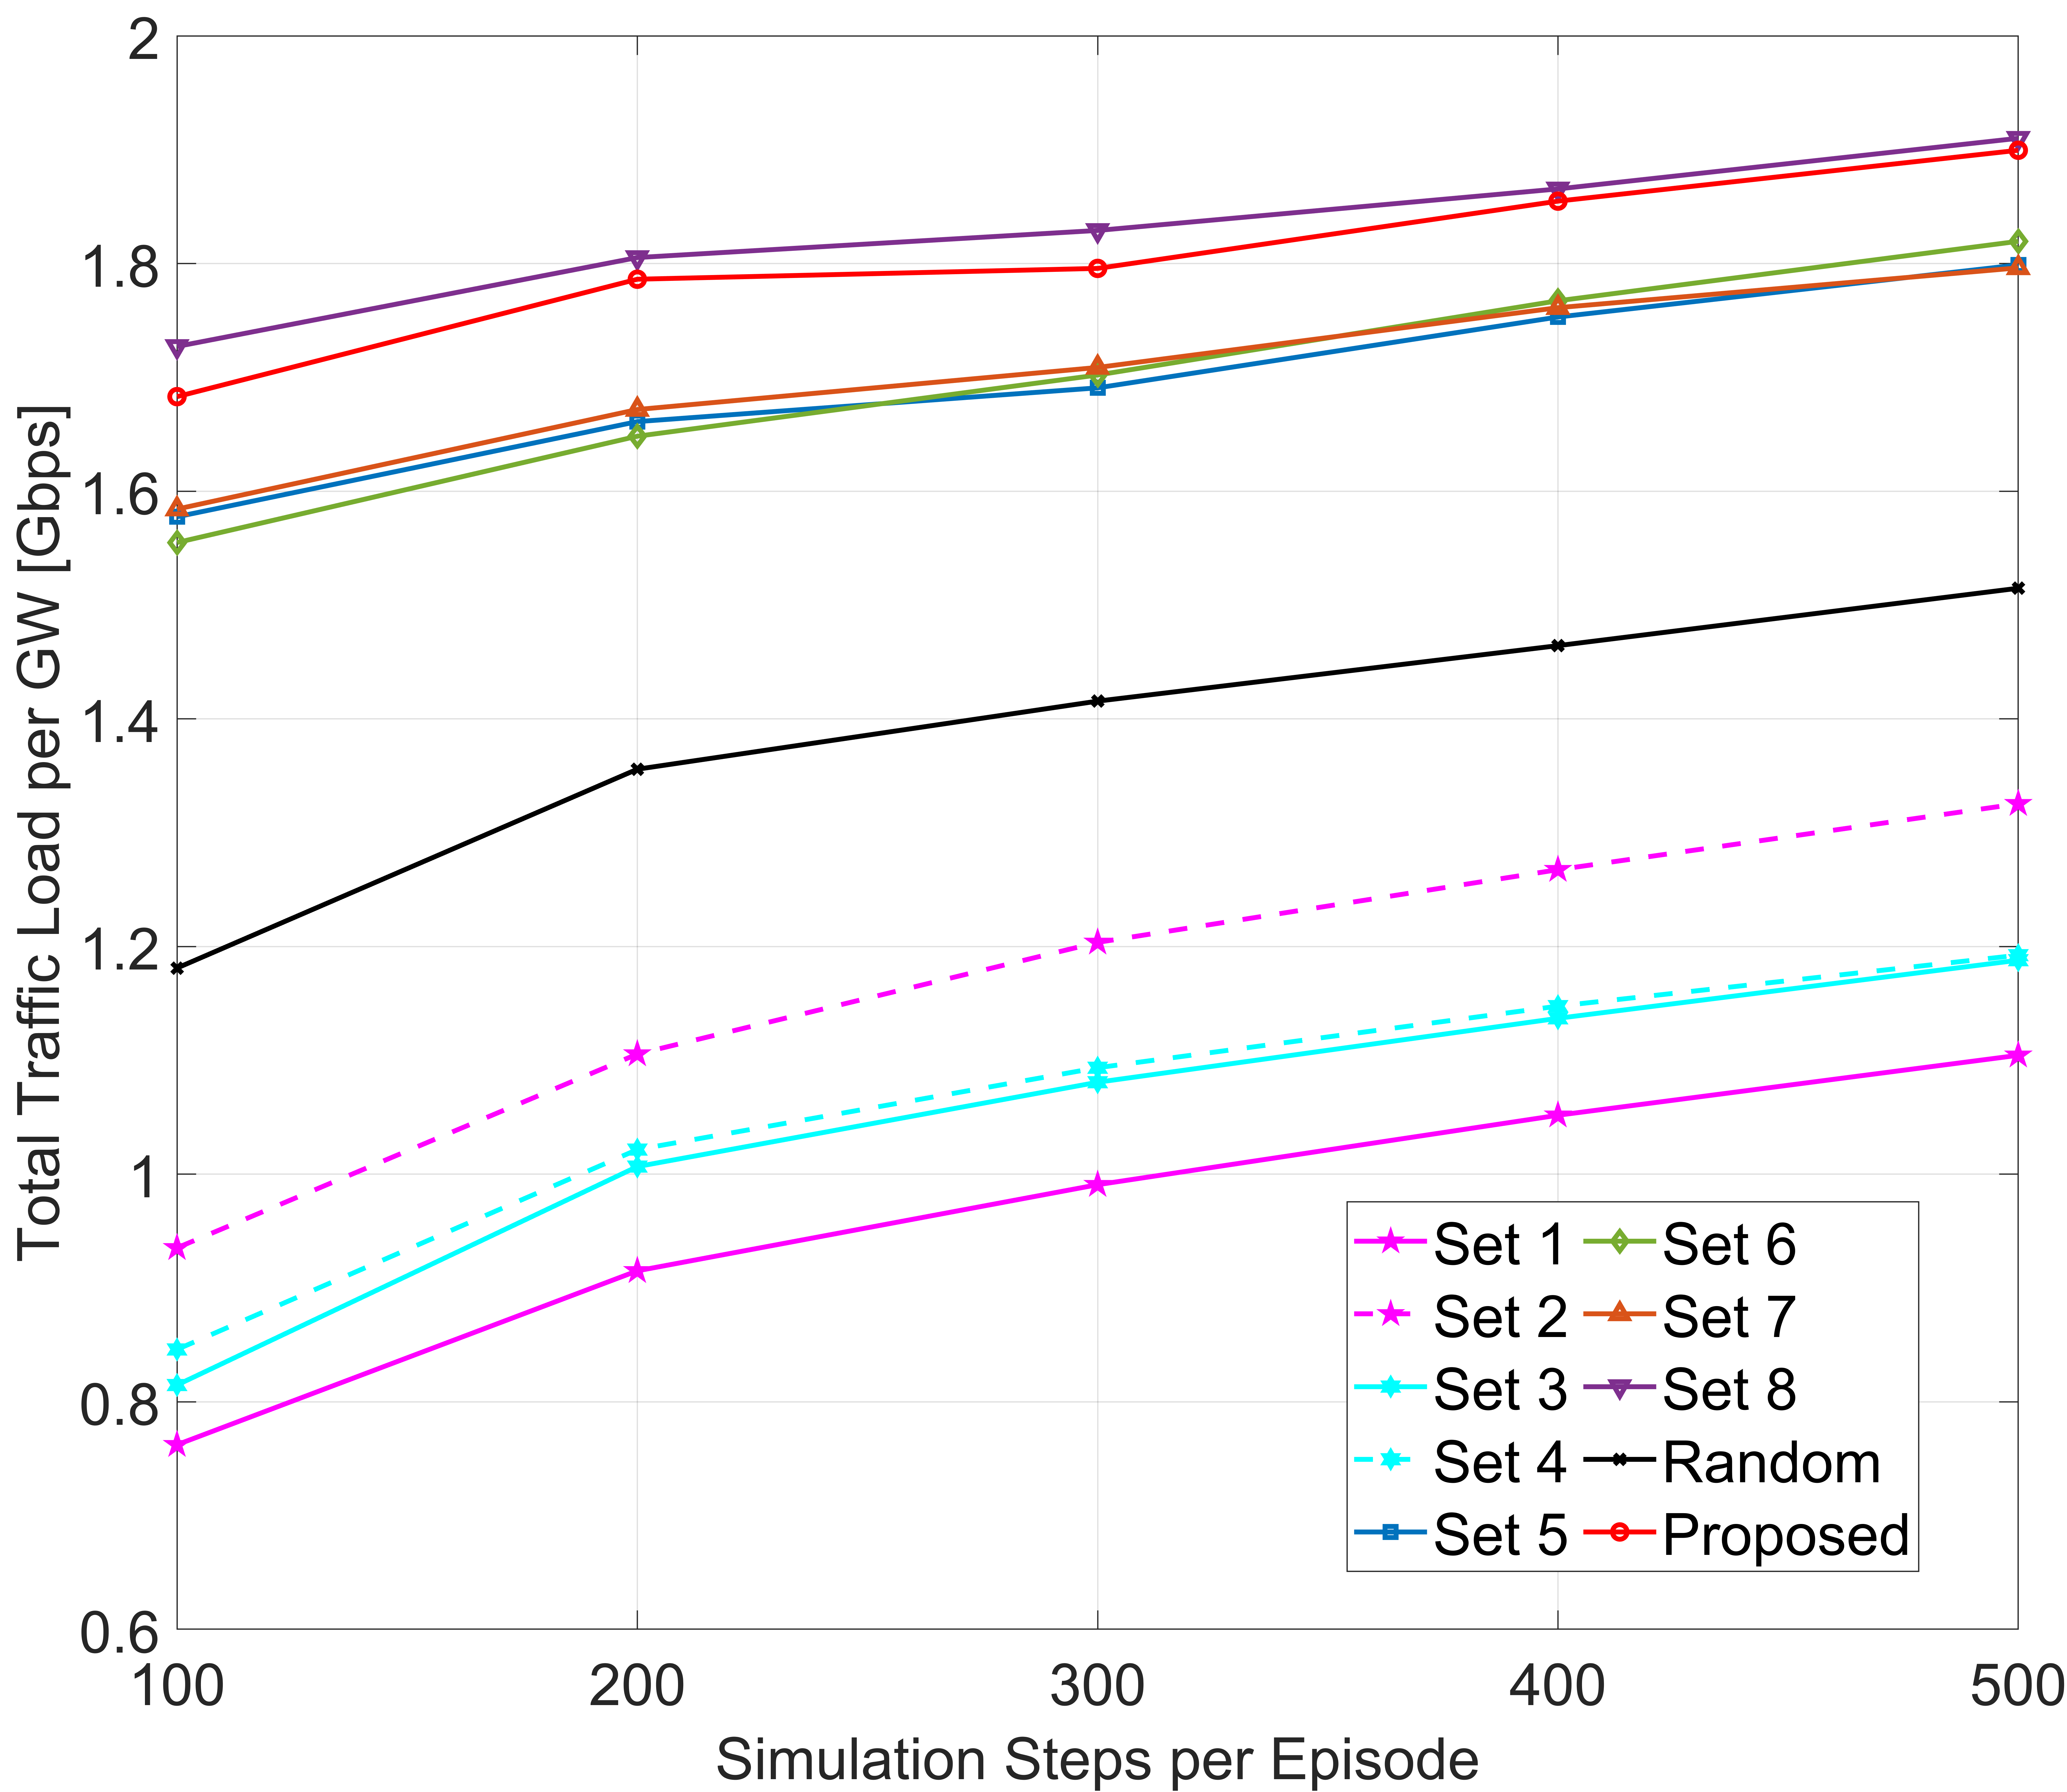
\includegraphics[width=\linewidth]{figure/6.traffic.png}
    \caption{Average total traffic load processed per GW for the proposed algorithm and baselines across different simulation steps.}
    \label{fig:6.traffic}
\end{figure}

Fig.~\ref{fig:6.traffic} shows the average traffic per GW link as the simulation length increases from 100 to 500 steps. For all algorithms the carried traffic grows steadily with time, and the relative order between the schemes is preserved across the entire range. Signal based hysteresis baselines in Set~1 and Set~2 occupy the lowest region of the plot. Their average traffic rises from roughly 0.76 to 1.10 and from 0.94 to 1.33 at 500 steps, which indicates that relying only on instantaneous signal strength does not fully utilise GW capacity. Distance driven heuristics in Set~3 and Set~4 deliver slightly higher traffic than Set~1 and Set~2. Their curves start near 0.81 and 0.85 at 100 steps and converge to about 1.19 at 500 steps. This suggests that geometric selection of GWs is somewhat more effective in filling the links but still leaves a noticeable margin compared with learning based controllers.RL baselines in Set~5, Set~6, and Set~7 constitute a higher traffic group. At 500 steps they maintain values between 1.80 and 1.82, which shows that these policies push a large amount of traffic toward the network edge. Set~8, which adds hard target updates to the learning pipeline, achieves the highest traffic among the baselines. Its average load increases from 1.73 at 100 steps to 1.91 at 500 steps. The Random policy yields intermediate traffic. It grows from about 1.18 at 100 steps to 1.51 at 500 steps, higher than the purely heuristic baselines yet clearly lower than the reinforcement learning family. The proposed algorithm consistently tracks the upper envelope of the learning based methods. It starts at 1.68 at 100 steps and reaches 1.90 at 500 steps, only slightly below Set~8 and above Set~5, Set~6, and Set~7. Combined with the FLSO and UFLSO results, this shows that the proposed controller is able to drive traffic through the GWs as aggressively as the strongest reinforcement learning variant while incurring significantly fewer switching operations. Hence the proposed scheme exploits GW capacity very efficiently without paying the high stability cost of the most aggressive strategies.


% 그림~\ref{fig:6.traffic}은 각 GW가 서비스하는 총 트래픽 양을 보여주며 네트워크 처리 용량에 대한 통찰력을 제공합니다. 휴리스틱 기준(Set~1, 3, 4)은 훨씬 낮은 트래픽 부하(1.36에서 1.53 범위)를 보여주며, 엄격한 핸드오버 규칙이 사용 가능한 지상 자원을 완전히 활용하지 못하여 잠재적인 서비스 차단 또는 미활용으로 이어진다는 것을 나타냅니다. 대조적으로 RL 기반 방법은 일반적으로 더 높은 처리량을 달성합니다. 특히 Set~8(w/o PA)은 가장 높은 트래픽 부하(1.905)를 기록하지만 앞서 논의한 바와 같이 이는 낮은 안정성 및 부하 불균형과 관련이 있어 높은 부하가 효율적인 분산보다는 특정 노드의 혼잡으로 인한 것일 가능성이 큽니다. 제안된 Dueling DDQN 알고리즘은 1.888의 거의 최적에 가까운 트래픽 부하를 달성하여 표준 DQN Set~5: 1.800 및 DDQN Set~6: 1.809를 능가합니다. 결정적으로 제안된 방법은 우수한 부하 공정성과 안정성을 유지하면서 이 높은 처리량을 달성하여 단순히 인기 있는 게이트웨이에 과부하를 주는 것이 아니라 활용도가 낮은 자원으로 트래픽을 라우팅함으로써 네트워크의 잠재 용량을 효과적으로 잠금 해제함을 확인시켜 줍니다.

\begin{figure}[t]
    \centering
    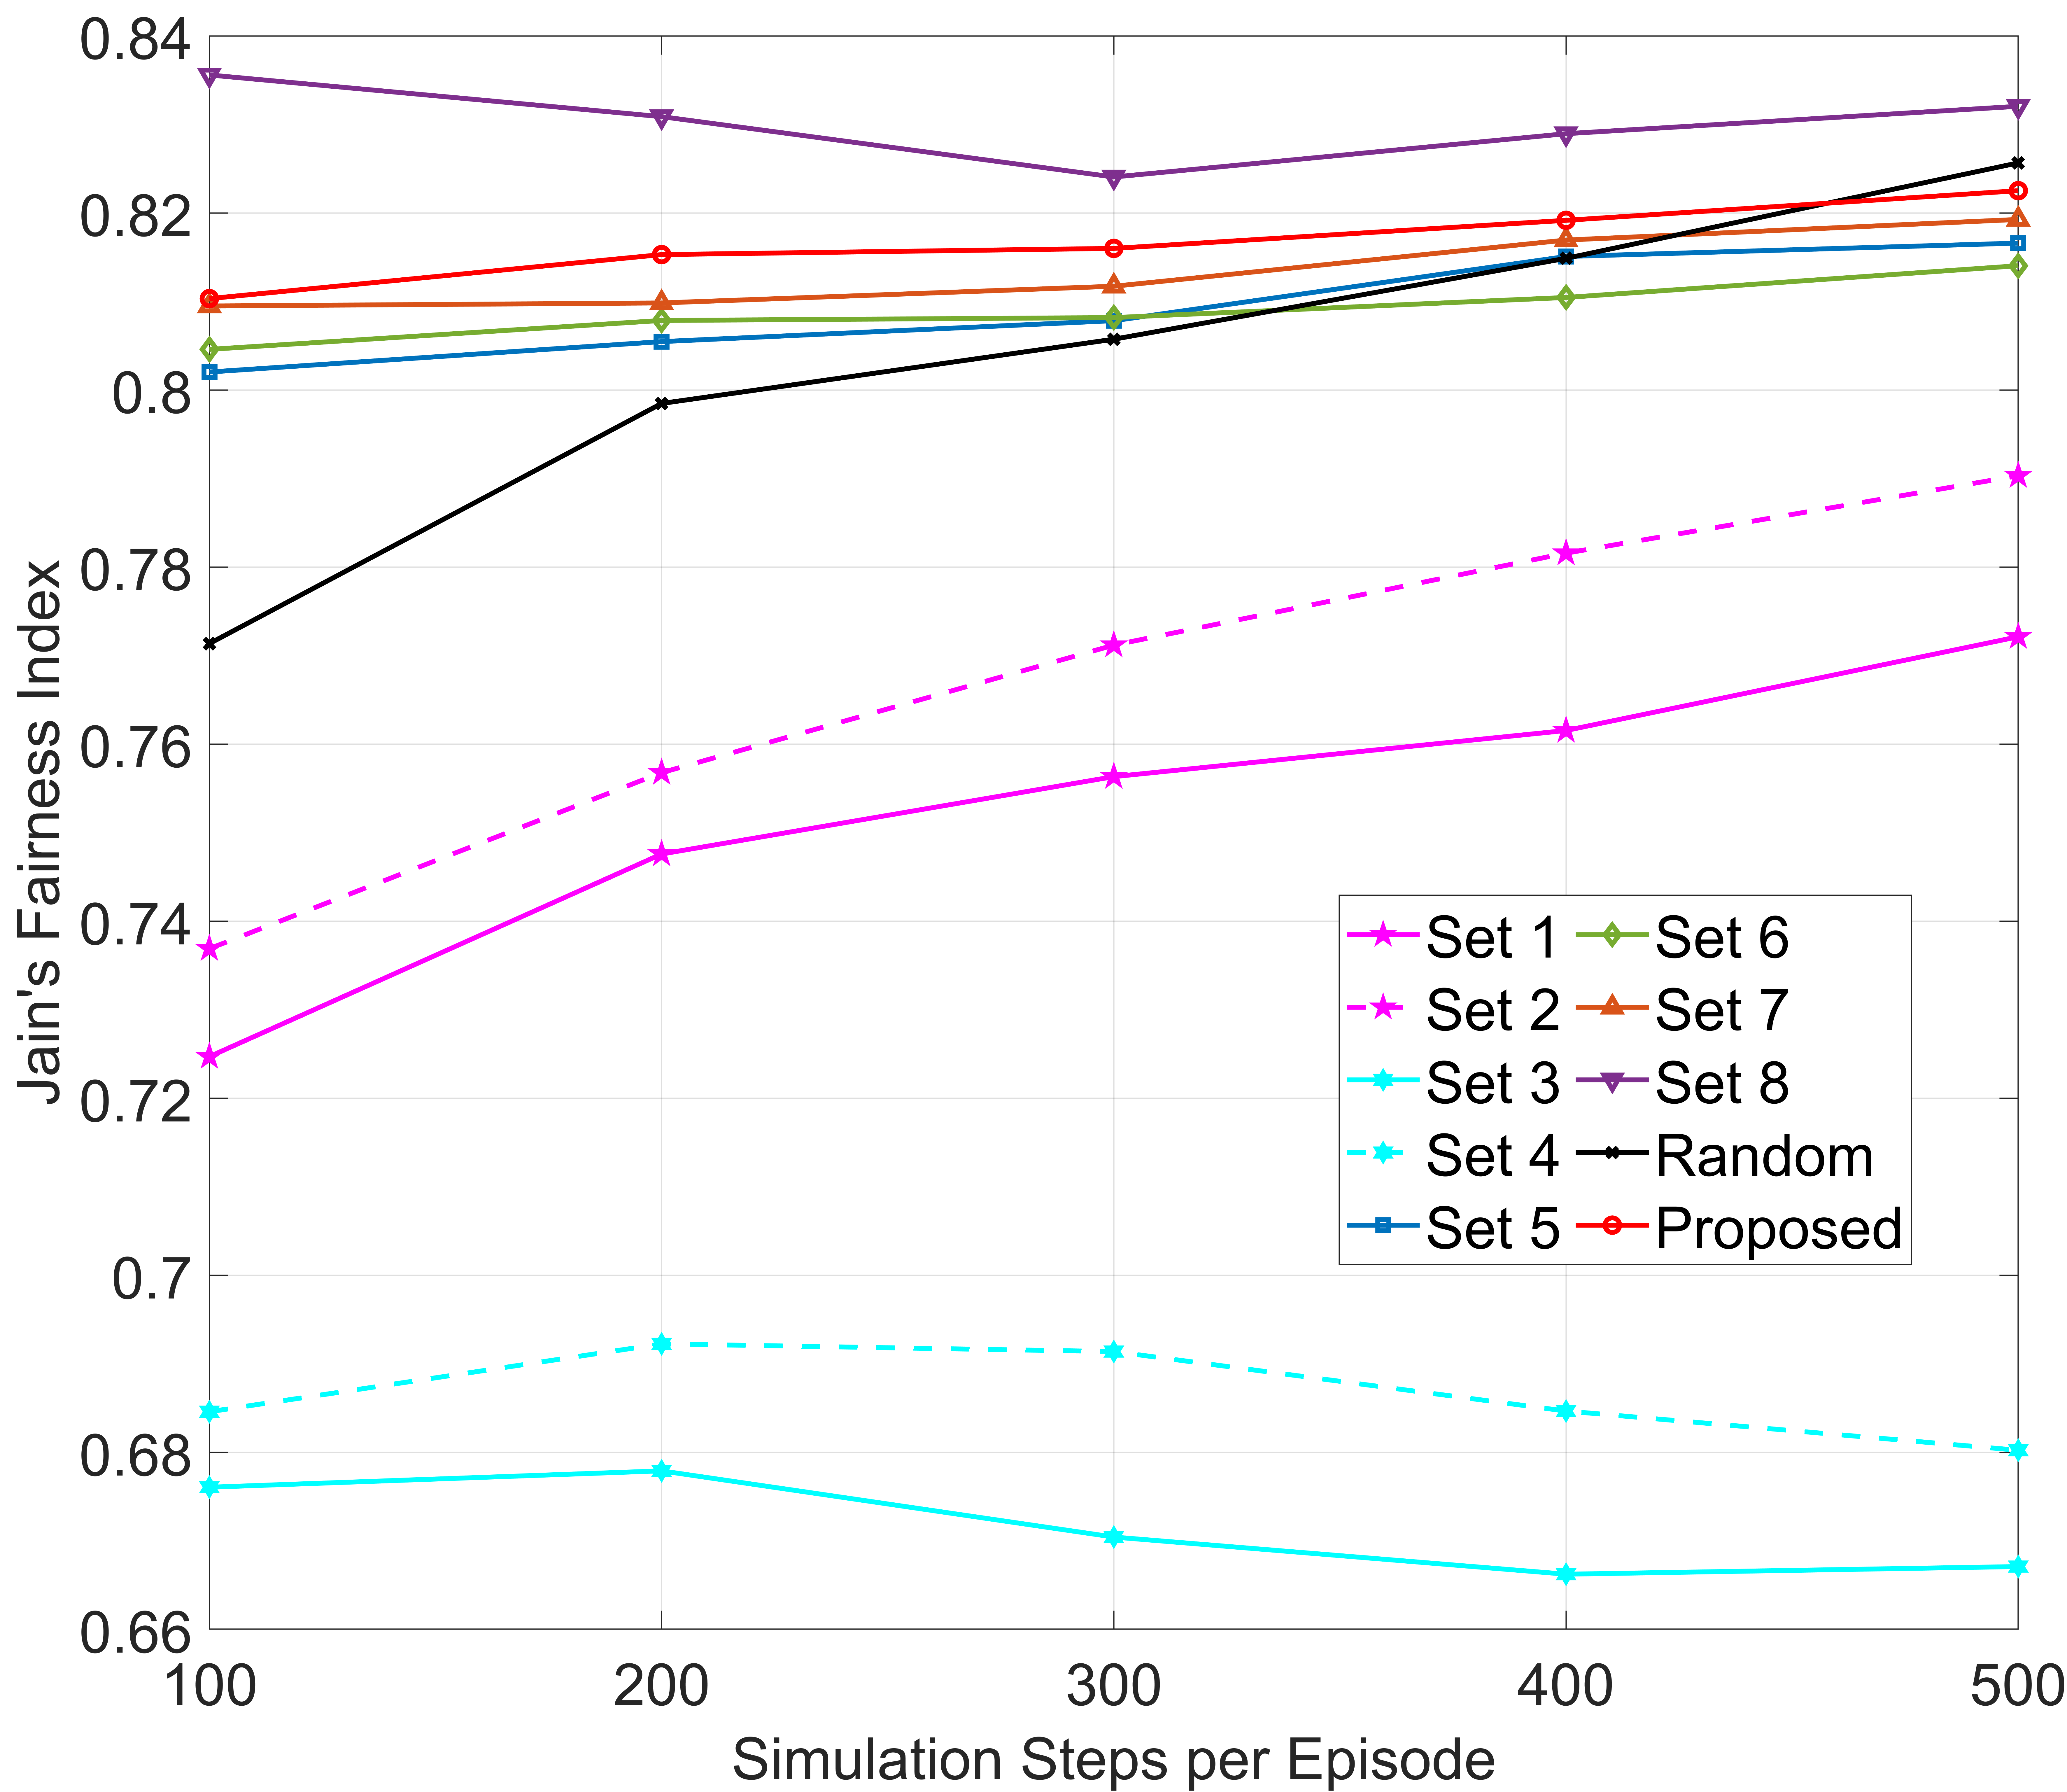
\includegraphics[width=\linewidth]{figure/7.jain.png}
    \caption{Average Jain's Fairness Index for the proposed algorithm and baselines across different simulation steps.}
    \label{fig:7.jain}
\end{figure}

Fig.~\ref{fig:7.jain} illustrates the evolution of the fairness index across GW links as the simulation progresses from 100 to 500 steps. For all algorithms the fairness remains relatively stable over time with gradual trends rather than abrupt changes. Distance based heuristics in Set~3 and Set~4 show the lowest fairness among all schemes. Their values stay around 0.67 across the simulation with a slight decrease toward the end. This indicates that purely geometric association tends to concentrate traffic on a subset of GWs and leaves others underutilised. Signal based methods in Set~1 and Set~2 achieve a moderate level of fairness. Their indices increase from roughly 0.72 to about 0.79 as the simulation length grows, which confirms that frequent signal driven switching helps redistribute traffic although the resulting balance is still limited compared with learning based strategies. The reinforcement learning baselines in Set~5, Set~6 and Set~7 form a high fairness group. Their values stay close to 0.80 throughout the simulation and converge to about 0.82 at 500 steps. The hard update variant in Set~8 reaches the highest fairness among all baselines, remaining around 0.83 over the whole time horizon. The Random policy also attains high fairness in a similar range, since randomised association tends to average out load over many GWs. The proposed algorithm starts from a fairness index of about 0.81 and gradually increases to approximately 0.82 at the final step. This places the proposed scheme in the same high fairness cluster as the strongest reinforcement learning baselines and the best performing baseline Set~8, while clearly outperforming the signal based and distance based heuristics. Together with the traffic and ToS results these observations confirm that the proposed controller not only carries a large amount of traffic but also distributes it evenly across GWs.

% \begin{table}[t]
% \centering
% \caption{FLSO statistics at 500 steps (mean with min–max bar).}
% \label{tab:flso_summary}
% \begin{tabular}{l c}
% \toprule
% Schemes & FLSO at 500 steps \\
% \midrule
% Set~1      & 16.99\;\flsobar{15.616}{16.993}{18.698} \\
% Set~2      & 11.55\;\flsobar{10.559}{11.547}{12.664} \\
% Set~3      &  8.73\;\flsobar{ 8.0095}{ 8.7302}{ 9.5860} \\
% Set~4      &  8.40\;\flsobar{ 7.3361}{ 8.3963}{ 9.4113} \\
% Set~5      &  7.95\;\flsobar{ 7.2010}{ 7.9503}{ 8.9736} \\
% Set~6      &  8.46\;\flsobar{ 7.8279}{ 8.4567}{ 9.1186} \\
% Set~7      &  7.75\;\flsobar{ 6.9786}{ 7.7483}{ 8.6643} \\
% Set~8      & 10.52\;\flsobar{ 9.4863}{10.5150}{11.4620} \\
% Random     &  7.96\;\flsobar{ 6.9396}{ 7.9617}{ 8.9956} \\
% Proposed   &  7.98\;\flsobar{ 7.3642}{ 7.9768}{ 8.6557} \\
% \bottomrule
% \end{tabular}
% \end{table}
